% !TeX root = cot_faith_arr.tex
% ============================================================
% ARR / ACL submission version.
%
% The 8-page limit covers the body only: Limitations, Ethics, References and
% Appendix are excluded. This file is the body. The unabridged manuscript --
% every per-family table, every null calibration, the four failed rollout-gate
% attempts, the judge validation -- is in arr_appendix.tex, generated verbatim
% from cot_faith_iclr.tex by scripts/build_arr_appendix.py so the two documents
% cannot drift apart. Nothing was cut to fit; it was moved.
%
% Build: latexmk -pdf cot_faith_arr.tex   (needs acl-style/ on TEXINPUTS)
% ============================================================
\documentclass[11pt]{article}

% acl.sty loads geometry itself (a4paper, margin=2.5cm). Loading geometry
% before it is a fatal Option Clash, which is why there is no \usepackage
% [margin=1in]{geometry} here as in the ICLR source.
\usepackage[review]{acl}

\usepackage{times}
\usepackage{latexsym}
\usepackage[T1]{fontenc}
\usepackage[utf8]{inputenc}
\usepackage{microtype}
\usepackage{booktabs}
\usepackage{amsfonts, amsmath, amssymb}
\usepackage{graphicx}
\usepackage{multirow}
% No inconsolata: it lives in texlive-fonts-extra, which the build image does
% not carry, and it only restyles \texttt. A cosmetic package that turns the
% submission build into a package-availability gamble is not worth the font.

\graphicspath{{figures/}}

% ---- Float placement -------------------------------------------------------
% Six body floats in eight two-column pages does not fit LaTeX's defaults, and
% the way it fails is silent. \dbltopfraction is 0.7, so a full-width float may
% occupy at most 0.7 x 704.6pt = 493pt of the page. fig:taxonomy is 387pt of
% artwork plus a ten-line full-width caption, which lands just over that line;
% it is refused, and because floats are placed strictly in order, every later
% figure* queues behind it. In the real submission the whole queue drained past
% the bibliography and printed on pages 41-44 of a 49-page PDF -- numbered,
% cross-referenced, and thirty-five pages from the text arguing from them.
%
% This was invisible upstream twice over: the 8-page metric is computed on the
% body-only build, whose \end{document} flushes the queue at page 8, and the
% engine emits no warning for a deferred float. bolt/run_arr_build.sh now reads
% float pages out of .aux and fails the job on this, so a regression is caught
% rather than submitted.
%
% These are the classic relaxed values, not arbitrary ones: allow a page to be
% mostly float (\textfraction 0.2 -> 0.05), allow a taller top float
% (\dbltopfraction 0.7 -> 0.9, which is what cleared fig:taxonomy while it was
% still in the submission and now keeps the appendix's own float queue draining
% on the page it was declared on), and let a float page be accepted when it is
% 70% rather than 50% full so a lone figure does not strand half a page of
% white. fig:taxonomy itself is now deferred for space -- see DEFERRED_FLOATS in
% scripts/build_arr_appendix.py -- but the values stay: the queue behaviour
% above is a property of the defaults and not of that one figure.
\renewcommand{\topfraction}{0.9}
\renewcommand{\dbltopfraction}{0.9}
\renewcommand{\bottomfraction}{0.5}
\renewcommand{\textfraction}{0.05}
\renewcommand{\floatpagefraction}{0.7}
\renewcommand{\dblfloatpagefraction}{0.7}
\setcounter{topnumber}{3}
\setcounter{dbltopnumber}{3}
\setcounter{totalnumber}{5}

% Shrink-to-fit, used by the generated appendix on every tabular.
%
% A bare \resizebox{\textwidth} would also ENLARGE a narrow table to full
% width, which is worse than the overflow it fixes. This measures first and
% scales only when the box is genuinely too wide, so a table that already fits
% is passed through at its natural size and untouched typographically.
% Standard LaTeX plus graphicx, which is already loaded -- no new package, and
% so no repeat of the inconsolata failure.
\newsavebox{\fitsavebox}
\newcommand{\fitwidth}[2]{%
  \sbox{\fitsavebox}{#2}%
  \ifdim\wd\fitsavebox>#1\relax
    \resizebox{#1}{!}{\usebox{\fitsavebox}}%
  \else
    \usebox{\fitsavebox}%
  \fi}

% No authblk, no titlesec, no \baselinestretch, no \parindent override: acl.sty
% fixes all of these and the ARR format check rejects deviations from them.

\title{CoT-Faith: A Benchmark for Chain-of-Thought Faithfulness\\
in Manipulation Vision-Language-Action Models}

\author{Anonymous ARR submission}

\begin{document}
\maketitle

\begin{abstract}
Vision-language-action models that emit chain-of-thought are proposed as a route to interpretable robotics, on the premise that the emitted reasoning drives the action. Every benchmark that tests that premise, ours included, scores an edit to the reasoning by the \emph{magnitude} of the action change it induces. \textbf{We show that this scoring rule has no construct validity}: on 12 of 12 configurations a meaning-preserving paraphrase moves the action \emph{more} than semantic edits do, swapping to a length-exact meaning-preserving floor flips the sign on all 12, and the two floors disagree by more than either disagrees with the semantic families, so neither licenses a claim about meaning. We establish this with \textbf{CoT-Faith}, one paired-intervention protocol applied uniformly to 15 manipulation VLAs in four model families over ten edit families and three calibration nulls: 324 scored (run, family) cells and $52{,}338$ released per-sample records. Four further measurements support that conclusion, each a way it could have failed. The score is close to a decode-collision counter ($R^2{=}0.93$ against $1 - P(\Delta{=}0)$ over 324 cells), so its advertised threshold-insensitivity follows from what it counts. Requiring the action change to point the \emph{implied} direction moves the top-ranked model from first of eight to seventh (Spearman $\rho = 0.48$). Attention mass on the CoT segment is pinned by architecture while causal effect spans $5.2\times$. And retraining one recipe unchanged moves the score $7.5\times$ further than resampling the decode does. Constructively, that direction-aware score is the one instrument here with a measured null: it clears its own floor on 7 of 11 configurations (by $6.2$--$11.1\times$ on our six LoRA and data variants and $3.0\times$ on ECoT-bridge), and correctly fails on a no-CoT control. We release all records and an audit script that checks 1,717 claims and fails on any mismatch.
\end{abstract}

\section{Introduction}
\label{sec:intro}

\begin{figure*}[t]
    \centering
    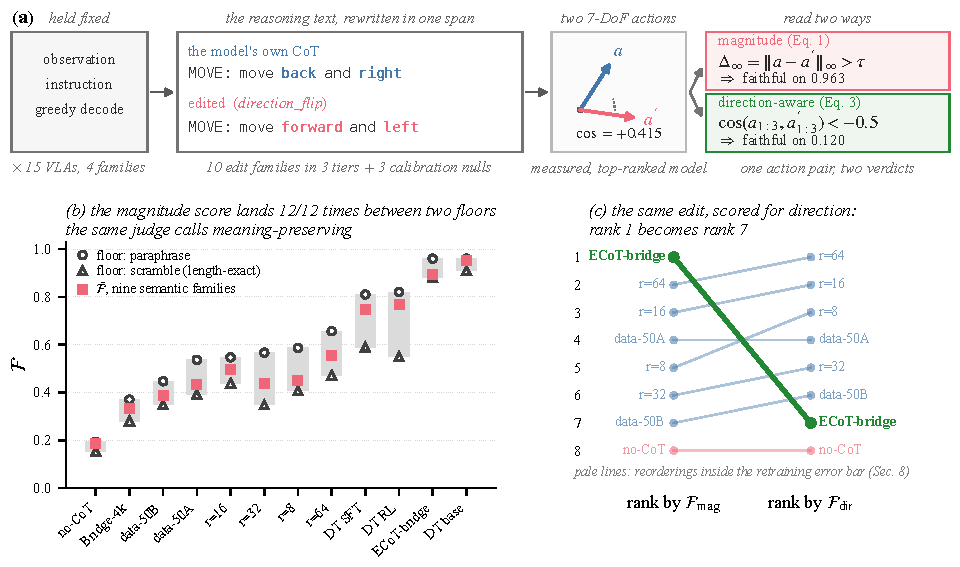
\includegraphics[width=\textwidth]{fig1_overview.pdf}
    \caption{\textbf{One observation, two reasoning traces, and two scoring rules that disagree about which model is most faithful.} \emph{(a)} The protocol (\S\ref{sec:benchmark}): observation, instruction and decode held fixed, the model's own CoT rewritten in one span, the two 7-DoF actions compared. The \texttt{MOVE} lines are the released \emph{direction\_flip} pair, highlighted by a word-level diff of it rather than by hand; the arrows are drawn at the top-ranked model's \emph{measured} mean translation cosine, $+0.415$, so after left$\leftrightarrow$right is reversed its action still points substantially the same way. Magnitude scoring calls that faithful on $0.963$ of samples; requiring the sign calls it faithful on $0.120$. \emph{(b)} Why no absolute $\mathcal{F}$ here is a quantity of faithfulness (\S\ref{sec:floors}): each column is one calibrated configuration, the grey band spans its two meaning-preserving floors as certified by the same blind judge, and the nine-family semantic mean falls \emph{inside} that band on 12 of 12, so which floor is nominated decides the sign of the result. \emph{(c)} The ranking that follows (\S\ref{sec:directional}): the magnitude score $\mathcal{F}_{\text{mag}}$ (Eq.~\ref{eq:faith}) on the left against $\mathcal{F}_{\text{dir}}$ (Eq.~\ref{eq:fdir}) on the right, both on \emph{direction\_flip} (Table~\ref{tab:directional}), the only family with an implied direction to require, so this is not the family-mean ordering of the leaderboard. Only the highlighted move is larger than the retraining error bar of \S\ref{sec:variance}: the model a leaderboard reader would pick goes from first to seventh of eight, while the pale reorderings are inside that bar and should not be read as ordered. Rank agreement is positive but weak (Spearman $\rho = 0.476$), i.e.\ the disagreement is concentrated at the top rather than spread over the cohort.}
    \label{fig:overview}
\end{figure*}

Vision-language-action (VLA) models that emit chain-of-thought reasoning alongside their action tokens are widely proposed as a route toward interpretable robotics: the reasoning is expected to expose the model's plan for review, correction, or safety monitoring \citep{ecot,cotvla,ecotlite,deepthinkvla}. This premise, that the emitted CoT \emph{drives} the subsequent action decode, underwrites CoT-based safety monitors, CoT-edit corrective interventions, and CoT-derived auditing. It has not been evaluated for manipulation VLAs under uniform conditions. Recent work evaluates CoT-faithfulness for driving VLAs \citep{vladrivebench,pinocchio} and probes CoT-based safety monitors in a small manipulation cohort \citep{doubleedged}; a cross-model, cross-corpus, standardized manipulation benchmark is missing.

We built one, applied it to 15 VLAs across 4 model families, and the result is one claim about the instrument rather than a set of findings about the models. \textbf{The magnitude-based edit score that this benchmark and every precedent we know of is built on does not measure faithfulness}: not noisily and not only for some models, but with no null it clears and with the sign of every result it produces decided by which meaning-preserving family is nominated as its floor (\S\ref{sec:floors}). Everything else here is evidence for that claim, and each strand is a way it could have failed. The score could have been measuring displacement badly, leaving the floor an offset to correct: it is close to a decode-collision counter, which is the mechanism (\S\ref{sec:collision}). No better rule might have existed, making the failure the question's rather than this score's: we build one that clears a null, and it disagrees at the top of the ranking, where a leaderboard is read (\S\ref{sec:directional}). The field's cheaper proxy could have been sound: attention on the CoT segment is pinned by architecture while causal effect spans $5.2\times$ (\S\ref{sec:dissociation}). And large gaps could have survived an uncalibrated score: retraining one recipe unchanged moves it $7.5\times$ further than the bar we submitted (\S\ref{sec:variance}). Figure~\ref{fig:overview} carries the claim and the first two strands.

\paragraph{Contributions.} The claim of \S\ref{sec:floors} is the contribution and \S\S\ref{sec:collision}--\ref{sec:variance} are the four strands that make it hard to escape. Two things support them. \textbf{The benchmark} (\S\ref{sec:benchmark}): ten edit families in a three-tier taxonomy plus three calibration nulls, on $\sim$100 LIBERO first-step samples per family per model, with an $N{=}100$ cross-corpus sweep on Bridge~V2, RT-1/Fractal and BC-Z, and a direction-aware score $\mathcal{F}_{\text{dir}}$, the one instrument here with a measured null, which is what we recommend an admission rule be built on rather than $\mathcal{F}$. \textbf{A release built to be checked} (\S\ref{sec:release}): all per-sample records, an audit script asserting 1,717 claims against them (field presence, not merely record counts), and an admission rule that rejects all eight of our own submissions.

\section{Related work}
\label{sec:related}

CoT-faithfulness in language models is measured by perturbing the reasoning and observing the answer \citep{lanham2023,turpin2023}, and the field's central finding is that stated reasoning frequently does not determine the output. Transferring that method to VLAs is attractive because the ``answer'' is a continuous action rather than a token, so the effect size is directly measurable. Two lines do this for driving \citep{vladrivebench,pinocchio}, and \citet{doubleedged} probes manipulation safety monitors under perturbation. All of them score an edit by the \emph{magnitude} of the induced change, which is what makes our result a claim about the shared rule rather than about our implementation of it. \S\ref{sec:floors} and \S\ref{sec:collision} argue that this scoring rule needs a per-model null before any of its outputs can be read; \S\ref{sec:directional} says what to use instead. Attention-based interpretability for VLAs \citep{ecot,cotvla} reports attention mass on the CoT segment; \S\ref{sec:dissociation} shows attention mass and edit response are dissociated, so neither substitutes for the other. Full discussion in Appendix~\ref{sec:appendix}.

\section{The CoT-Faith benchmark}
\label{sec:benchmark}


\paragraph{Protocol.} For each sample $s$ and edit family $f$ we decode greedily twice (once on the model's own CoT, once on the edited CoT), holding the observation, the instruction and the decode fixed, and compare the two 7-DoF actions:
\begin{equation}
\Delta_\infty^{s,f} = \max_{i \in [7]}\bigl|\,a_i(s, f(\text{cot}_s)) - a_i(s, \text{cot}_s)\,\bigr|,
\label{eq:delta}
\end{equation}
with $a_i$ normalized to $[-1,1]$. A sample is faithful under $f$ iff $\Delta_\infty^{s,f} > \tau$, $\tau = 0.05$, and
\begin{equation}
\mathcal{F}(m,f) = \tfrac{1}{N}\textstyle\sum_s \mathbf{1}[\Delta_\infty^{s,f}(m) > \tau].
\label{eq:faith}
\end{equation}
This is a paired intervention: it references no ground-truth demonstration, so it is defined even on a policy that performs the task poorly, a property that matters in \S\ref{sec:release}. Figure~\ref{fig:frames} shows what one such edit does over a whole rollout, and what the policy read while it did.

\paragraph{Edit families.} Thirteen families: ten in three tiers (structural, word-level, object/causal) and three calibration nulls. The nulls make a score interpretable and are the part of the design we would keep if we kept nothing else: \emph{paraphrase\_null} (meaning-preserving synonym swap); \emph{bbox\_jitter\_null} (meaning-preserving numeric perturbation); and an out-of-CoT control, \emph{instr\_random\_sub}, which corrupts five \emph{instruction} tokens and never touches the reasoning. A fourth control is filed with the ten: \emph{selfsplice\_control}, an identity substitution, which must score $0$ and does, on 11/11 CoT-VLAs; the judge export names it \emph{identity\_control} and groups it with the nulls, so the two names are one family and the judge scores 12 of the 13. A blind LLM judge (\texttt{Qwen2.5-7B-Instruct}, in neither architecture family under test; full protocol, blinding and skip accounting in Appendix~\ref{sec:judge_edits}), itself gated on an identity control ($1.000$) and a pooled negative control ($0.175$), validates the generators over 437 pairs: \emph{paraphrase\_null} preserves meaning at $0.975$ and \emph{bbox\_jitter\_null} at $1.000$, so the floors are validated rather than asserted. It also found one family's name oversells it: \emph{adversarial\_plausible} is judged plausible on only $0.125$ of pairs, corrected in the taxonomy (Appendix~\ref{sec:appendix}).

\paragraph{Direction-aware score.} Eq.~\ref{eq:delta} credits movement in \emph{any} direction. For families whose semantics imply a signed consequence we require the sign. After \emph{direction\_flip} reverses left$\leftrightarrow$right / up$\leftrightarrow$down / in$\leftrightarrow$out,
\begin{align}
\mathcal{F}_{\text{dir}} &= \tfrac{1}{N}\textstyle\sum_s \mathbf{1}\!\left[c^f_s < -0.5\right], \label{eq:fdir}\\
c^f_s &= \cos\bigl(a_{1:3}(s,\text{cot}_s),\, a_{1:3}(s,f(\text{cot}_s))\bigr) \nonumber
\end{align}
with analogous criteria for \emph{gripper\_flip} and \emph{negation}. It needs no new inference: it reuses action pairs we already release.

\paragraph{Models.} 15 VLAs: 4 OpenVLA non-CoT baselines, 3 DeepThinkVLA variants (base/SFT/RL, a PaliGemma-based second architecture family with a different reasoning format and action tokenizer), 1 public ECoT-bridge, and 7 LoRA fine-tunes of our own isolating rank, data quantity, and reasoning-target training. Every trained configuration was trained \emph{twice} at a byte-identical recipe, which supplies the error bar that matters (\S\ref{sec:variance}).

\section{The claim: the magnitude score has no null it clears}
\label{sec:floors}

A faithful model should be \emph{insensitive} to an edit that preserves meaning, so $\mathcal{F}$ on \emph{paraphrase\_null} is a \emph{floor} a faithful model should stay \emph{under}, not a lower bound on anything good. Write $\bar{\mathcal{F}}$, or $\bar{\mathcal{F}}_{\text{mag}}$ where the contrast with $\mathcal{F}_{\text{dir}}$ must be marked, for the mean of $\mathcal{F}$ over the semantic families; the quantity of interest is the floor-corrected $\bar{\mathcal{F}}_{\text{diff}} = \bar{\mathcal{F}}(\text{semantic}) - \mathcal{F}(\text{floor})$. A \emph{ceiling} is always a maximum-effect reference an edit is compared up to: \emph{cross\_task\_swap} for $\mathcal{F}$, and for $\mathcal{F}_{\text{dir}}$ the largest score over the families with no direction to reverse (\S\ref{sec:directional}).

\textbf{It is negative on 12 of 12 configurations} (Table~\ref{tab:floors}), across both architecture families, with $\bar{\mathcal{F}}_{\text{diff}}$ from $-0.139$ to $-0.006$. A meaning-preserving synonym swap moves the action \emph{more reliably} than a semantic edit does, on every full-CoT model we measured. On our strongest model a paraphrase changes the action $94.7\%$ of the time against $96.3\%$ for replacing the entire trace with an unrelated task's reasoning, our designated maximum-effect control. The one positive entry in our calibration set is off this table: the retrained no-CoT variant ($+0.014$), trained on an action-only target, which is where a floor-corrected statistic \emph{should} return its own floor. It is the protocol's positive control, not a model that passes.

\textbf{The effect is per-task, not an artifact of averaging}, the inferential statistic Table~\ref{tab:floors}'s point estimates lack. Recomputing $\mathcal{F}$ \emph{within} each of the $85$ LIBERO-90 episode files every leaderboard row was scored on, from the released records and with no new inference (Table~\ref{tab:per_task}), the semantic mean is below that task's own paraphrase floor on more tasks than above it on all $8$ configurations, an exact two-sided binomial test on the untied tasks giving $p$ from $9.0{\times}10^{-11}$ to $0.020$ on the seven full-CoT rows: all seven survive Holm correction across the eight tests at $\alpha{=}0.05$. The eighth row is the no-CoT control and is null ($25$ below, $29$ above, $p = 0.683$), which is the row that should not separate. The claim is about this fixed set of $85$ tasks, not about LIBERO-90 as a population.

\paragraph{The obvious repair does not work, and why it fails is the real result.} \emph{paraphrase\_null} is the one family in our taxonomy that changes sequence length: its synonym table contains multi-word expansions (\emph{release} $\to$ ``let go of''), and it changes word count on 38/40 judged heads by a mean of $+0.97$ words, while \emph{direction\_flip}, \emph{negation}, \emph{syntactic\_scramble} and \emph{bbox\_jitter\_null} change it on 0/40. So the floor may be subtracting a length effect. \textbf{We did not test this before submission.} The control that settles it is \emph{syntactic\_scramble}: the same judge scores it meaning-preserving at $1.000$, and it is length-exact by construction.

Against that floor, $\bar{\mathcal{F}}_{\text{diff}}$ is \emph{positive} on 12/12: \textbf{the sign flips on every single configuration.} That alone would license switching floors and reporting the favourable sign. What forbids it is the third statistic: \textbf{on 12/12 configurations the gap between the two floors exceeds the gap between the semantic mean and \emph{either} floor.} At $r{=}32$ the floors are $0.567$ and $0.348$, a spread of $0.219$, while the semantic mean $0.438$ lies \emph{between} them, $0.129$ and $0.090$ away. Two edits our validated judge certifies as meaning the same thing disagree with each other more than either disagrees with edits that change meaning.

\textbf{We therefore report both floors everywhere and treat the magnitude metric as uninformative about meaning in either direction}: a weaker claim than our submitted one, and the one the data supports. Swapping floors would only trade one unlicensed sign for its opposite.

\paragraph{A third floor, and it lies outside the CoT.} \emph{instr\_random\_sub} corrupts five \emph{instruction} tokens and never touches the reasoning, so it bounds how much of any edit score is CoT$\to$action routing rather than generic prompt sensitivity. The specificity ratio $\bar{\mathcal{F}}/\mathcal{F}(\emph{instr\_random\_sub})$ exceeds $1$ on $5$ of the 12 configurations, so on those the semantic families do move the action more reliably than a corrupted instruction. But the margins are $+0.083$, $+0.074$, $+0.025$, $+0.014$ and $+0.009$ in $\bar{\mathcal{F}}$, and retraining the same recipe moves $\bar{\mathcal{F}}$ by up to $0.092$ (\S\ref{sec:variance}): \textbf{no configuration in this benchmark clears its own out-of-CoT control by more than its own retraining noise.} The public checkpoint is below the control ($0.878$) and so is the entire second architecture family ($0.996$, $0.806$, $0.814$). We report this control on every row for that reason, and would require it of any submission.

\begin{table}[t]
\centering\small
% 26.68pt over the 218pt column at \tabcolsep 3.2pt. Padding first, scaling
% second: seven columns means fourteen gaps, so 3.2 -> 2.0pt reclaims 16.8pt
% of pure whitespace, and \fitwidth then absorbs the ~10pt remainder at a ~4%
% shrink instead of the ~12% it would need on its own. \fitwidth measures
% before it scales, so if a later edit narrows this table it is passed through
% untouched rather than blown up to fill the column.
\setlength{\tabcolsep}{2.0pt}
\renewcommand{\arraystretch}{1.08}
\fitwidth{\columnwidth}{%
\begin{tabular}{@{}l rr r rr r@{}}
\toprule
& \multicolumn{2}{c}{floor $\mathcal{F}$} & &
  \multicolumn{2}{c}{$\bar{\mathcal{F}}_{\text{diff}}$ vs.\ floor} & \\
\cmidrule(lr){2-3}\cmidrule(lr){5-6}
Model & para & scram & $\bar{\mathcal{F}}$ & para & scram &
  $|\text{p}-\text{s}|$ \\
\midrule
\texttt{no-CoT}      & $0.193$ & $0.154$ & $0.187$ & $-0.006$ & $+0.034$ & $0.039$ \\
\texttt{r=8}         & $0.587$ & $0.408$ & $0.448$ & $-0.139$ & $+0.040$ & $0.179$ \\
\texttt{r=16}        & $0.547$ & $0.438$ & $0.494$ & $-0.053$ & $+0.056$ & $0.109$ \\
\texttt{r=32}        & $0.567$ & $0.348$ & $0.438$ & $-0.129$ & $+0.090$ & $0.219$ \\
\texttt{r=64}        & $0.657$ & $0.472$ & $0.554$ & $-0.102$ & $+0.083$ & $0.185$ \\
\texttt{data-50A}    & $0.537$ & $0.391$ & $0.435$ & $-0.102$ & $+0.043$ & $0.145$ \\
\texttt{data-50B}    & $0.447$ & $0.348$ & $0.385$ & $-0.061$ & $+0.037$ & $0.099$ \\
\texttt{ECoT-bridge} & $0.960$ & $0.880$ & $0.894$ & $-0.066$ & $+0.014$ & $0.080$ \\
\addlinespace[2pt]\midrule\addlinespace[2pt]
\texttt{DT base}     & $0.960$ & $0.910$ & $0.951$ & $-0.009$ & $+0.041$ & $0.050$ \\
\texttt{DT SFT}      & $0.810$ & $0.590$ & $0.748$ & $-0.062$ & $+0.158$ & $0.220$ \\
\texttt{DT RL}       & $0.820$ & $0.550$ & $0.767$ & $-0.053$ & $+0.217$ & $0.270$ \\
\addlinespace[2pt]\midrule\addlinespace[2pt]
\texttt{Bridge-4k}$^\dagger$ & $0.370$ & $0.280$ & $0.332$ & $-0.038$ & $+0.052$ & $0.090$ \\
\midrule
\multicolumn{4}{@{}l}{\emph{all 12 configurations}}
  & \textbf{$-$ 12/12} & \textbf{$+$ 12/12} & \textbf{12/12} \\
\bottomrule
\end{tabular}}
\caption{\textbf{Both meaning-preserving floors, on every configuration we can calibrate.} $\bar{\mathcal{F}}$ is the mean over the nine semantic families, the \emph{cross\_task\_swap} ceiling and the out-of-CoT \emph{instr\_random\_sub} control among them; the appendix averages the seven core families instead, which lowers every value by $0.004$--$0.048$ ($\bar{\mathcal{F}}_{\text{diff}}$ then runs $-0.013$ to $-0.180$) and leaves the 12/12 result below intact. The sign of $\bar{\mathcal{F}}_{\text{diff}}$ is decided entirely by which meaning-preserving family is nominated as the floor: negative against \emph{paraphrase\_null} on 12/12, positive against the length-exact \emph{syntactic\_scramble} on 12/12. Both are certified meaning-preserving by the same blind judge ($0.975$, $1.000$), whose protocol is Appendix~\ref{sec:judge_edits}. The last column adds no third finding: given the two signs it is their sum, so it exceeds both by construction. What it supplies is the \emph{size} of the problem on all 12 at once, which is what makes both floors unusable rather than one of them correct. Bottom row: the count over all 12, not a mean. $^\dagger$the 4k Bridge-subset deconfound checkpoint, included because it calibrates but excluded from every leaderboard cell: on the samples it scores as faithful, $90\%$ move the single gripper bit and nothing else, and its mean per-axis translation change is $20\times$ smaller than ECoT-bridge's ($0.010$ against $0.197$), so its $\mathcal{F}$ is not on the same scale as the other rows.}
\label{tab:floors}
\end{table}

\section{Why it fails: the score is a collision counter}
\label{sec:collision}

\begin{figure*}[t]
    \centering
    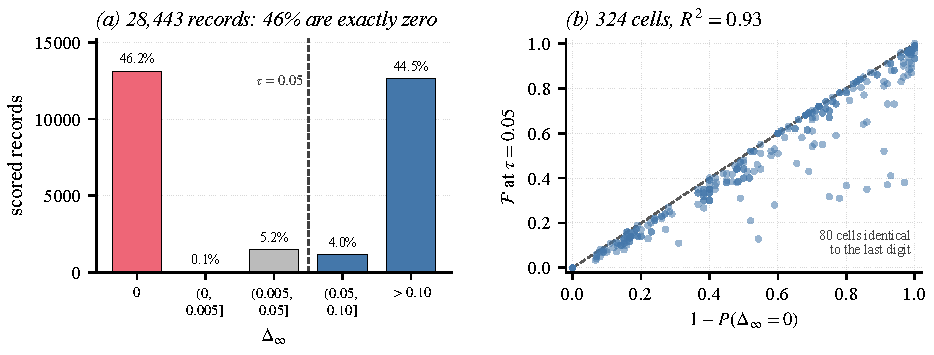
\includegraphics[width=\textwidth]{fig13_collision.pdf}
    \caption{\textbf{$\mathcal{F}$ is close to a decode-collision counter.} \emph{(a)} The per-sample $\Delta_\infty$ distribution over the $28{,}443$ scored records of the 30 runs here (one seed each) is bimodal: a spike at exactly zero and a broad mode well above $\tau$, with little mass near the threshold itself. That empty neighbourhood is what makes $\mathcal{F}$ insensitive to $\tau$. \emph{(b)} The same fact stated as an identity: across the 324 (run, family) cells with $n \geq 20$, $\mathcal{F}$ at $\tau{=}0.05$ falls on the line $1 - P(\Delta_\infty{=}0)$ at $R^2 = 0.926$. Threshold-insensitivity is a consequence of this, not independent evidence that the metric is robust.}
    \label{fig:collision}
\end{figure*}

Were the floor failure an offset to correct, $\mathcal{F}$ would still be measuring displacement. It barely does. The per-sample $\Delta_\infty$ distribution is strongly bimodal: over the $28{,}443$ scored records of the 30 runs covered here (one seed per configuration) $46.2\%$ are \emph{exactly} zero (the argmax over action bins landed on the identical bin despite a different prompt) and $44.5\%$ exceed $0.10$. Of the records that move at all, only $9.8\%$ land below $\tau$, and if almost no mass lies near the threshold then $\mathcal{F}$ is close to $1 - P(\Delta_\infty = 0)$: not a measure of how far the action moved, but a count of how often the decode failed to collide.

That is measurable, so we measured it (Figure~\ref{fig:collision}). Across the 324 (run, family) cells with $n \geq 20$, $\mathcal{F}$ at $\tau{=}0.05$ tracks $1 - P(\Delta_\infty{=}0)$ at $r = 0.963$, $R^2 = 0.926$, with 80 cells identical to the last digit; per configuration the agreement is $R^2 = 0.972$. \textbf{Threshold-insensitivity is a consequence of the metric being nearly a collision counter, not evidence that it is robust.} This invalidates no comparison here (a collision rate is well-defined and self-consistent, and every $\mathcal{F}$ we report is computed the same way), but it changes what the quantity is called, and it is the mechanism behind \S\ref{sec:floors}: a score whose dynamic range is dominated by argmax collisions has no particular reason to separate meaning-changing from meaning-preserving edits, and it does not. We release $P(\Delta_\infty{=}0)$ beside $\mathcal{F}$ for all 324 cells in the release.

\section{Direction-aware scoring: the top of the ranking inverts, and this instrument has a null}
\label{sec:directional}

\begin{table}[t]
\centering\small
% 14.56pt over the column. Same treatment as tab:floors: 4 -> 2.6pt of padding
% over fourteen gaps reclaims ~19pt, which covers it outright, and \fitwidth
% is the guard rather than the fix -- it measures first and only scales if a
% future edit pushes this back over.
\setlength{\tabcolsep}{2.6pt}
\renewcommand{\arraystretch}{1.08}
\fitwidth{\columnwidth}{%
\begin{tabular}{@{}l c@{\ }l c c@{\ }l c@{}}
\toprule
& \multicolumn{2}{c}{magnitude} & &
  \multicolumn{2}{c}{direction-aware} & \\
\cmidrule(lr){2-3}\cmidrule(lr){5-6}
Model & $\mathcal{F}_{\text{mag}}$ & {\footnotesize$\pm$sd} & rank
      & $\mathcal{F}_{\text{dir}}$ & {\footnotesize$\pm$sd} & $\cos$ \\
\midrule
\texttt{ECoT-bridge} & \textbf{0.963} & {\footnotesize$.006$} & \textbf{1}
  & 0.120 & {\footnotesize$.043$} & $\mathbf{+0.415}$ \\
\texttt{r=64}     & 0.823 & {\footnotesize$.016$} & 2
  & \textbf{0.779} & {\footnotesize$.021$} & $-0.509$ \\
\texttt{r=16}     & 0.749 & {\footnotesize$.028$} & 3
  & 0.666 & {\footnotesize$.045$} & $-0.320$ \\
\texttt{data-50A} & 0.699 & {\footnotesize$.022$} & 4
  & 0.642 & {\footnotesize$.011$} & $-0.256$ \\
\texttt{r=8}      & 0.696 & {\footnotesize$.041$} & 5
  & 0.649 & {\footnotesize$.020$} & $-0.313$ \\
\texttt{r=32}     & 0.652 & {\footnotesize$.024$} & 6
  & 0.579 & {\footnotesize$.028$} & $-0.147$ \\
\texttt{data-50B} & 0.639 & {\footnotesize$.022$} & 7
  & 0.542 & {\footnotesize$.013$} & $-0.111$ \\
\texttt{no-CoT}   & 0.274 & {\footnotesize$.042$} & 8
  & 0.087 & {\footnotesize$.021$} & $\mathbf{+0.759}$ \\
\bottomrule
\end{tabular}}
\caption{\textbf{Magnitude vs.\ direction-aware faithfulness on \emph{direction\_flip}.} $\mathcal{F}_{\text{mag}}$ is Eq.~\ref{eq:faith}, $\mathcal{F}_{\text{dir}}$ is Eq.~\ref{eq:fdir}, and $\cos$ is the mean cosine between the original and post-edit xyz translation, so a faithful model is \emph{negative} and the two bold positive entries are the two models that move the same way after the direction is reversed. Every row is a 3-sampling-seed mean; $\pm$sd is the seed std, printed here so the reader can apply the caveat rather than take it on trust. The \emph{rank} column orders $\mathcal{F}_{\text{mag}}$ and exists only to make the inversion legible: ranks 4 and 5 are separated by less than either row's seed std, and no adjacent pair among ranks 2--7 is separated by more than the retraining bar of \S\ref{sec:variance}, so none of them should be read as ordered. The gap between the magnitude and direction blocks is the point: the top row of one is the second-from-bottom of the other, $0.659$ against seed stds of $0.006$ and $0.021$. Computed from the released action pairs with no new inference; per-family means in Appendix~\ref{sec:appendix}.}
\label{tab:directional}
\end{table}

\textbf{The ranking reverses at the top.} ECoT-bridge, numerically highest in every magnitude column, has $\mathcal{F}_{\text{mag}} = 0.963 \pm 0.006$ on \emph{direction\_flip} but $\mathcal{F}_{\text{dir}} = 0.120 \pm 0.043$, with mean translation cosine $+0.415$: \textbf{it moves in substantially the \emph{same} direction after the direction is reversed}. The LoRA variants it outscores by $1.2$--$1.5\times$ on magnitude genuinely reverse ($\cos$ from $-0.111$ to $-0.509$) and outscore it by $4.5$--$6.5\times$ on $\mathcal{F}_{\text{dir}}$. The inversion dwarfs the seed noise producing it: ECoT-bridge's deficit against $r{=}64$ is $0.659$ against per-row seed stds of $0.043$ and $0.021$.

\textbf{We state the disagreement as one number, and it is smaller than ``the ranking inverts'' would suggest.} Over the eight leaderboard configurations the two orderings correlate at Spearman $\rho = 0.476$ (Kendall $\tau_b = 0.500$; 21 concordant against 7 discordant pairs), positive on all three sampling seeds ($0.400$--$0.500$). At $n{=}8$ that estimate carries a Fisher-$z$ 95\% interval of $[-0.34, 0.88]$, which spans $0$: \textbf{eight configurations cannot establish how well the two rules agree in general}, and we claim no such thing. What they can establish is the disagreement itself, a single reordering larger than the error bar of \S\ref{sec:variance} rather than a correlation: the two rules do not reverse the cohort wholesale, they disagree almost entirely about one configuration, which shifts 6 rank positions while no other shifts more than 2. That is the worse case for a leaderboard, not the milder one, since the one row a reader would act on is the row the two rules cannot agree about, and it is why we publish no ranking: publishing either order would be a choice of conclusion rather than a measurement.

\textbf{$\mathcal{F}_{\text{dir}}$ is also the one instrument here that clears a null}, and this is the constructive half of the paper. Our own critique of the field is that edit sensitivity gets reported without a null, and $\mathcal{F}_{\text{dir}}$ was introduced to show the top of the ranking inverts without itself being calibrated. So we calibrated it against the \emph{ceiling}: the largest $\mathcal{F}_{\text{dir}}$ any of the eight families with no left$\leftrightarrow$right semantics reaches, namely both meaning-preserving floors (\emph{paraphrase\_null}, \emph{syntactic\_scramble}), \emph{bbox\_jitter\_null}, the out-of-CoT \emph{instr\_random\_sub}, the \emph{cross\_task\_swap} ceiling, \emph{verb\_swap}, \emph{subject\_swap} and \emph{negation}. None gives a model any reason to \emph{reverse} a translation vector, so their maximum is a floor for the treatment to clear. Two of the eight are in against our own interest: \emph{cross\_task\_swap} is the maximum-effect family in the benchmark and \emph{negation} carries a signed criterion of its own (\S\ref{sec:benchmark}), so both can only push the ceiling up.

\begin{table}[t]
\centering\small
% Same padding treatment as the other two body tables: six columns over a
% 218pt column needs the 4pt default trimmed, and \fitwidth is the guard
% rather than the fix.
\setlength{\tabcolsep}{3.0pt}
\renewcommand{\arraystretch}{1.08}
\fitwidth{\columnwidth}{%
\begin{tabular}{@{}l c c c l c@{}}
\toprule
Config & $\mathcal{F}_{\text{dir}}$ & $N$ & ceiling
       & ceiling family & $\times$ \\
\midrule
\texttt{r=64}        & 0.779 & 299 & 0.070 & {\footnotesize\emph{cross\_task}} & \textbf{11.1} \\
\texttt{data-50B}    & 0.582 & 299 & 0.057 & {\footnotesize\emph{cross\_task}} & \textbf{10.3} \\
\texttt{r=32}        & 0.589 & 299 & 0.077 & {\footnotesize\emph{negation}}    & \textbf{7.7} \\
\texttt{r=8}         & 0.666 & 299 & 0.093 & {\footnotesize\emph{cross\_task}} & \textbf{7.1} \\
\texttt{r=16}        & 0.672 & 299 & 0.097 & {\footnotesize\emph{verb\_swap}}  & \textbf{7.0} \\
\texttt{data-50A}    & 0.659 & 299 & 0.107 & {\footnotesize\emph{cross\_task}} & \textbf{6.2} \\
\texttt{ECoT-bridge} & 0.120 & 299 & 0.040 & {\footnotesize\emph{cross\_task}} & \textbf{3.0} \\
\midrule
\texttt{no-CoT}      & 0.087 & 299 & 0.113 & {\footnotesize\emph{cross\_task}} & 0.8 \\
\texttt{DT RL}       & 0.010 & 100 & 0.020 & {\footnotesize\emph{paraphrase}}  & 0.5 \\
\texttt{DT SFT}      & 0.010 & 100 & 0.050 & {\footnotesize\emph{negation}}    & 0.2 \\
\texttt{DT base}     & 0.000 & 100 & 0.000 & {\footnotesize\emph{paraphrase}}  & --- \\
\bottomrule
\end{tabular}}
\caption{\textbf{The one instrument in this paper with a measured null.} $\mathcal{F}_{\text{dir}}$ on \emph{direction\_flip} against the \emph{ceiling} it has to clear: the maximum $\mathcal{F}_{\text{dir}}$ over the eight families with no left$\leftrightarrow$right semantics, enumerated in the text and including two that can only raise it, none of which gives a model any reason to reverse a translation vector. $\times$ is treatment over ceiling. The seven rows above the rule clear; the four below do not, and \textbf{that a null control is among them is the result, not a gap}: \texttt{no-CoT} sits \emph{below} its own ceiling, which is what a calibrated instrument should do to an ablation with no CoT to be faithful to. \texttt{DT base} reverses on no family at all, so its ratio is $0/0$ and undefined rather than large. The ceiling family is named per row because it is not constant, and a ceiling fixed at one family would be a weaker null. $N$ is samples pooled across the three sampling seeds, so these are not Table~\ref{tab:directional}'s 3-seed means: same records, aggregated as the null requires, since a per-seed ceiling is a maximum over eight noisier estimates and biases the ceiling up.}
\label{tab:fdirnull}
\end{table}

Table~\ref{tab:fdirnull} is that calibration. On the six CoT-trained LoRA and data variants \emph{direction\_flip} clears the ceiling by $\mathbf{6.2}$--$\mathbf{11.1\times}$ and ECoT-bridge clears it at $3.0\times$, which is the $0.96 \to 0.12$ collapse seen from the null side, \textbf{while the no-CoT control sits \emph{below} its own ceiling}, the one trained-cohort configuration that does not clear, and exactly the behaviour a calibrated instrument should show. $\mathcal{F}_{\text{mag}}$ fails that same test: on the no-CoT control it reads $0.187$ against a $0.193$ floor, so magnitude scoring cannot separate the ablation from the models it ablates and the direction check can. All three DeepThinkVLA checkpoints return $\mathcal{F}_{\text{dir}} \leq 0.010$ and do \emph{not} clear, so the second architecture family fails outright; we report that as a negative row, not as coverage. \textbf{7 of 11 configurations clear their own null.} An admission rule should be built on this, not on $\mathcal{F}_{\text{mag}}$, whose floor question \S\ref{sec:floors} shows to be unanswerable in either direction.

\section{No cheaper proxy: attention and causal effect are dissociated}
\label{sec:dissociation}

% A 3.2:1 three-panel figure cannot go in a 218pt column: at \columnwidth it
% renders 68pt tall and sets its tick labels at roughly 3pt, which is not
% readable on paper. It was \columnwidth because the body was 8/8 pages and a
% figure* costs more; the float fix bought a page back, so it can be set at the
% width its aspect ratio requires. The audit asserts the height still fits
% under \dbltopfraction.
\begin{figure*}[t]
    \centering
    
\includegraphics[width=\textwidth]{fig4_dissociation.pdf}
    \caption{\textbf{Attention mass and causal effect are dissociated.} \emph{(a)} Attention on the CoT segment is $\in [0.335, 0.358]$ across all 8 variants, a max--min gap of $2.30$\,pp, only $1.2\times$ the $1.95$\,pp worst same-config retraining gap (grey band), so these are ties, not an ordering. The \texttt{no-CoT} control is one of the 8: trained action-only, it still attends to its unused CoT span at $0.3491$, within $0.002$\,pp of \texttt{data-50B}, whose causal effect in (b) is $2.1\times$ higher. \emph{(b)} The same models' mean faithful rate over the 7 non-control edit families spans $5.2\times$. \emph{(c)} Normalizing each model by its own \emph{cross\_task\_swap} ceiling leaves $1.9\times$, so most but not all of (b) is a per-model scale effect. Early layers $L=\{0,1,2,3\}$; depth sweep below.}
    \label{fig:dissociation}
\end{figure*}

If attention on the CoT segment tracked the causal effect of editing it, a monitor could read the cheaper signal. It does not. Attention over the visual, instruction, CoT and previous-action segments splits $\approx 0.29/0.30/0.34/0.07$ on all 8 ECoT-family CoT-VLAs, regardless of training regime, against $0.52/0.42/0.00/0.05$ on the OpenVLA non-CoT baselines: \textbf{attention on the CoT segment is a floor set by architecture, and reasoning-target training moves it by little}. Causal effect is not: $\bar{\mathcal{F}}_{\text{mag}}$ spans $5.2\times$ over the same models (Figure~\ref{fig:dissociation}), so a monitor reading the first is not reading the second. \textbf{The pinning is a property of the architecture and not of the corpus.} Running the public checkpoint over Bridge~V2, RT-1/Fractal and BC-Z at $N{=}100$ each, distinct embodiments with the CoT self-generated because none ships annotations, every attention bucket lands within $2.1$\,pp of its LIBERO value and all but BC-Z's CoT bucket within $0.9$\,pp; the edit response transfers too, over a $0.06$ range on \emph{direction\_flip} (Appendix~\ref{sec:cross_corpus}). The nulls were not run there, so that is portability of the pipeline, not evidence about those corpora.

Two limits, both measured. The attention claim is an \emph{early-layer} claim: a 5-layer-set $\times$ 3-seed sweep has $\alpha(\text{cot})$ leads in exactly 1 of the 4 four-layer blocks probed (the one we report) and swings $18.7$\,pp across depth against a worst-case sampling $\sigma$ of $0.26$\,pp. No bucket ordering should be reported without its layer set. And on the second architecture family $\alpha(\text{cot})$ is \emph{never} the largest bucket on any checkpoint, so ``the CoT bucket is largest'' is specific to both the layer set and the family.

Nor does attention predict \emph{failure}, in domain and in robot units after withdrawing a cross-domain version for a protocol error: $\alpha(\text{cot})$ gives AUROC $0.596$ with a CI spanning chance on one model at $N{=}153$, and we do not generalize it (Table~\ref{tab:p3}).

\section{No margin to spare: the error bar is the retraining, not the seed}
\label{sec:variance}

An uncalibrated score can still order models if the gaps are large enough. They are not. All leaderboard rows are 3-seed means with Wilson 95\% CIs (half-widths $\leq 0.067$). \textbf{This does not fix the problem it appears to fix.} Sampling seeds hold the checkpoint fixed. So we trained all seven configurations a second time at a byte-identical recipe, scoring each replicate on the same 100 samples with byte-identical interventions. Each pair is two different models: on $r{=}32$ the \emph{unedited} action differs on 66 of 100 samples. Of the three ways of asking how much a number moves when nothing is done to it, resampling the decode from a \emph{frozen} checkpoint, the bar we submitted, is smallest; retraining the \emph{same} config is $7.5\times$ larger, and the between-variant spread a reader would want to interpret only $1.2\times$ that, which is why we report no within-family ordering. In $\mathcal{F}$, the unit the leaderboard is read in, per-family $\mathcal{F}$ moves across the pairs by up to $\mathbf{0.260}$, which is about $3.9\times$ that widest Wilson half-width, and $\bar{\mathcal{F}}$ by up to $0.092$, which is $1.4\times$ it and larger than most between-model differences in the table. Taking the worst of the $9$ families compared per pair (\emph{data-50A}'s worst is a control, so the bound is conservative), six of seven pairs move it past that half-width: single-family differences below ${\sim}0.26$ are not model differences. The controls behave throughout (\emph{selfsplice\_control} is $0.000$ in all 14 runs), so this is variance in the measured quantity, not the harness. \emph{Compute.} Every trained checkpoint is a LoRA fine-tune of the same 7B ECoT-OpenVLA for $15{,}000$ steps at batch size $2$ in bf16, $14$ runs in all; per-run wall-clock is not in our artifacts, so we quote the recipe rather than a GPU-hour figure. \emph{Multiplicity.} We report each test rather than a corrected family, with one exception: the $8$ per-task tests of \S\ref{sec:floors} carry a headline, and there we state the Holm-corrected outcome.

\section{Release and audit}
\label{sec:release}

We release $52{,}338$ per-sample edit records ($45{,}989$ scored), $3{,}620$ attention records (the first $20$ per run where the aggregate is over $100$; that prefix reproduces the full-$N$ bucket ordering to within $\mathbf{0.37}$\,pp), the decoder audits, and every script, with the generators, the judge prompt and a datasheet carrying the per-asset upstream licence table, under a permissive licence: $53.9$\,MB of self-contained JSON that re-derives every number here with no network access. Our audit script asserts \textbf{1,717 claims} against the artifacts, treats a missing artifact as a failure, not a skip, and exits non-zero on any mismatch.

Two disclosures the audit forced, both unwelcome. \textbf{First, it now checks what records \emph{contain}, not only how many there are}, because the count-only version passed $869/869$ while the release paragraph made a false claim about its own schema. It immediately found a second instance: 438 scored records (the three cross-corpus runs) carry deltas without the action pair or edit metadata, so those runs are reproducible at aggregate level only. \textbf{Second, six of the eight leaderboard rows come from a policy whose single-step open-loop prediction does not beat a constant}: its L$_1$ is $0.0486$ against $0.0457$ for predicting the per-dimension dataset mean, in every frame the checkpoint ships. This does not invalidate $\Delta_\infty$, which is a self-comparison referencing no ground truth. It does mean those rows are edit-sensitivity measurements on weak policies, and it is the direct cause of the missing rollout evidence: at 40 episodes per arm both the clean-CoT and no-CoT arms score $0/40$, and a second run adds a \emph{direction\_flip} arm at $0/9$ against the same controls, so an edit-induced $\Delta$SR is undefined rather than zero and the harness reports none. The rollout does show the edit protocol running closed-loop, and it bounds something the first-step protocol cannot see: $381$ edits were skipped mid-rollout for want of a direction word to reverse.

Our leaderboard's admission rule requires a per-model paraphrase floor and a direction check. \textbf{It admits none of our own eight submissions}: all eight now carry a floor, and all eight score below it ($\bar{\mathcal{F}}_{\text{diff}}$ from $-0.028$ to $-0.179$), the highest-scoring one with a floor at the same height as its ceiling. That rule, rather than any score it admits, is the part of this work we expect to outlast the rest.


\section{Conclusion}

CoT-Faith set out to rank manipulation VLAs by how much their reasoning drives their actions. It cannot, and the obstacle is the scoring rule the whole line of work rests on: \textbf{magnitude-based edit scoring has no construct validity}. It clears no null, its sign is decided by which meaning-preserving family is nominated as the floor, and the four measurements we added to test that verdict sustain it: it is largely a decode-collision counter, the attention proxy that might have replaced it is dissociated from it, the gaps it reports are mostly narrower than the retraining variance nobody measures, and the one rule here that clears a null disagrees with it at the top of the ranking. Published faithfulness gaps obtained by magnitude scoring may survive neither check, and measuring the floor should precede reporting the score.

\section*{Limitations}

The full list is Appendix~\ref{sec:appendix}; the load-bearing items: \emph{Construct validity fails on 11 of 12 calibration entries} (a row set that differs from Table~\ref{tab:floors}'s twelve by one checkpoint each way), and the exception is a negative control, so no absolute $\mathcal{F}$ here is a measure of faithfulness.

\emph{Our one constructive result is confounded with policy competence.} The six configurations that clear the $\mathcal{F}_{\text{dir}}$ null at $6.2$--$11.1\times$ are exactly the six whose open-loop prediction does not beat a constant (\S\ref{sec:release}), and the one strong policy clears at $3.0\times$: this design does not separate ``reverses the vector when the reasoning says to'' from ``is a weak policy''. An isotropic action distribution scores $0.25$ at our $\cos < -0.5$ criterion, so its absolute values are not effect sizes either, and every ceiling in Table~\ref{tab:fdirnull} sits far below $0.25$, i.e.\ these action changes are strongly clustered, not random.

\emph{No number here is rollout-conditioned.} The leaderboard is first-step; the paired rollout returns $0/40$ in both arms, a checkpoint-competence problem rather than a compute or suite-availability one, so an edit-induced $\Delta$SR is undefined and none is reported. The rollout harness, its arm-pairing diagnostics and the trajectory-level readout we substituted for SR are in the full-length manuscript. \emph{P3 is one model with a negative result} supporting no cross-model comparison. \emph{Attention claims are early-layer claims} and do not survive the depth sweep. \emph{Per-family $N$ varies from 58 to 100} with a visibility gate, so each model is compared only against its own floor and ceiling. \emph{$\mathcal{F}_{\text{dir}}$ does not transfer to the second architecture family}: all three DeepThinkVLA checkpoints fail it. \emph{OpenVLA-OFT is excluded} after failing to load at its authors' declared pins.

\section*{Ethics Statement}

The motivation is a safety concern: CoT-based monitors and CoT-edit interventions are proposed for deployed robots on the assumption that the reasoning is load-bearing, and our results indicate that the standard test of that assumption does not measure what it claims to. The negative result is the safety-relevant contribution, and \S\ref{sec:floors} withdraws a headline we submitted rather than overclaim the other way.

All experiments are in simulation (LIBERO) or on public offline corpora: no physical robot was operated, and no human subjects or personal data involved. We release measurement records, not new capability. Upstream licenses are resolved from the Hugging Face Hub API rather than from memory and released machine-readably; 3 of the 15 assets declare no license upstream, and we grant no rights to them rather than assign a license we cannot verify. The release states the uses it does not support, including that no number in it is rollout-conditioned and that the leaderboard is a diagnostic, not a ranking. The blind judge that certifies both floors is an LLM run as a method component (\texttt{Qwen2.5-7B-Instruct}, locally, under a fixed released prompt gated on two controls; \S\ref{sec:benchmark}); every number here is produced by the released scripts and re-checked by the audit.

% Flush every pending body float before the bibliography. Without this the
% four body figures survived the float queue all the way into the appendix and
% printed on page 41 of the 49-page submission -- present, numbered, cross-
% referenced, and forty pages from the text that argues from them. The
% body-only build placed them at pages 6-8, so this was invisible in the
% page-count metric the build job reports and only showed up on the real PDF.
\clearpage
\bibliographystyle{acl_natbib}
% Extracted verbatim from cot_faith_iclr.tex by hand-run; the ARR body
% and the full-length version must cite the same entries.
\begin{thebibliography}{99}
% Bibliography provenance. Every entry below is checked against a live registry by
% experiments/verify_citations.py, whose report is released as
% results_v2/canonical_runs/citation_check/citation_check.json and asserted by
% scripts/verify_paper_numbers.py. That check found six real defects on its first run:
% five entries printed exactly five authors joined by "and" -- reading as complete lists
% where the registry gives 7, 7, 7, 11 and 14 -- and one carried our own shorthand
% "(OpenVLA-OFT)" inside the registered title. All six are corrected below.
%
% All 51 of 51 entries CONFIRM on title, author-surname order and year against
% export.arxiv.org. Two obstacles had to be removed to get there, and both were
% ours rather than the registries'.
%
% (1) An accidental precondition. The check only queried arXiv when the entry itself
% printed an arXiv id, so venue-only citations (datasheets, cotvla, turpin2023,
% libero, colosseum) were unverifiable because of our formatting, not because of
% theirs. They are now resolved by exact-title search. The search accepts a hit only
% on an exact normalized-title match, never on arXiv's relevance rank, because
% confirming a citation against a neighbouring paper is worse than leaving it
% unconfirmed. Six candidate additions did not resolve exactly and were replaced by
% resolvable equivalents rather than written from memory.
%
% (2) Rate limiting, which appeared only when the bibliography grew. arXiv answers
% HTTP 429 above one request per three seconds. At 15 entries the run finished inside
% that window; at 51 it tripped the limit on 26 of them, and because the client
% counted any HTTP status as "registry reachable", the report showed arXiv up while
% 26 entries sat UNVERIFIED -- entries nobody had managed to ask about, filed as
% though they had been asked. The client now waits between calls, retries a 429, and
% records rate limiting as its own state, which the audit asserts against.
%
% DBLP was never the answer. It returns "CONNECT tunnel failed, 403" from the
% authoring network -- a proxy host allowlist, not throttling; doi.org,
% api.crossref.org, api.openalex.org, aclanthology.org, openreview.net and
% scholar.google.com are blocked the same way -- and times out on the TLS handshake
% from bolt task qrpd3f8z58, so falling back to it resolved nothing from anywhere.
%
% [VERIFY] datasheets: arXiv 1803.09010 confirms the title, all seven authors in order,
% and the comment "Published in CACM in December, 2021" (consistent with volume 64(12)).
% Volume, page range 86-92 and doi:10.1145/3458723 are still unresolved -- CHECK them
% against the publisher record before submission.
\bibitem[Gebru et~al.(2021)]{datasheets} T.~Gebru, J.~Morgenstern, B.~Vecchione, J.~Wortman~Vaughan, H.~Wallach, H.~Daum\'e~III, and K.~Crawford. Datasheets for datasets. \emph{Communications of the ACM}, 64(12):86--92, 2021.
\bibitem[Zawalski et~al.(2024)]{ecot} M.~Zawalski, W.~Chen, K.~Pertsch, O.~Mees, C.~Finn, and S.~Levine. Robotic control via embodied chain-of-thought reasoning. \emph{CoRL}, 2024. arXiv:2407.08693.
\bibitem[Chen et~al.(2025)]{ecotlite} W.~Chen, S.~Belkhale, S.~Mirchandani, O.~Mees, D.~Driess, et~al. Training Strategies for Efficient Embodied Reasoning. arXiv:2505.08243, 2025.
\bibitem[Yin et~al.(2025)]{deepthinkvla} C.~Yin, Y.~Lin, W.~Xu, S.~Tam, X.~Zeng, et~al. DeepThinkVLA: Enhancing Reasoning Capability of Vision-Language-Action Models. arXiv:2511.15669, 2025.
\bibitem[Zhao et~al.(2025)]{cotvla} Q.~Zhao, Y.~Lu, M.~J.~Kim, Z.~Fu, et~al. {CoT-VLA}: Visual Chain-of-Thought Reasoning for Vision-Language-Action Models. \emph{CVPR}, 2025.
\bibitem[Kim et~al.(2025)]{openvlaoft} M.~J.~Kim, C.~Finn, and P.~Liang. Fine-Tuning Vision-Language-Action Models: Optimizing Speed and Success. arXiv:2502.19645, 2025. Referred to as OpenVLA-OFT.
\bibitem[Turpin et~al.(2023)]{turpin2023} M.~Turpin, J.~Michael, E.~Perez, and S.~R.~Bowman. Language models don't always say what they think: unfaithful explanations in chain-of-thought prompting. \emph{NeurIPS}, 2023.
\bibitem[Lanham et~al.(2023)]{lanham2023} T.~Lanham et~al. Measuring faithfulness in chain-of-thought reasoning. arXiv:2307.13702, 2023.
\bibitem[Nguyen et~al.(2026)]{vladrivebench} T.~Nguyen, D.~Guo, T.~Lampo, F.~Wu, and B.~Yaman. {VLADriveBench}: Evaluating CoT-Action Relationship in VLA for Autonomous Driving. arXiv:2606.12706, 2026.
\bibitem[Foutter et~al.(2026)]{pinocchio} M.~Foutter, M.~Cercola, L.~Wild, Y.~Wang, M.~Li, et~al. Do vision-language-action models mean what they say? On the role of faithfulness in embodied reasoning. arXiv:2607.04681, 2026.
\bibitem[Trinh et~al.(2026)]{doubleedged} T.~D.~Trinh, N.~Akhtar, and B.~Azam. Reasoning as a double-edged sword: architecture and cross-stage robustness in vision-language-action models. arXiv:2607.17786, 2026.
\bibitem[Liu et~al.(2023)]{libero} B.~Liu, Y.~Zhu, C.~Gao, Y.~Feng, Q.~Liu, Y.~Zhu, and P.~Stone. {LIBERO}: Benchmarking Knowledge Transfer for Lifelong Robot Learning. \emph{NeurIPS Datasets \& Benchmarks Track}, 2023.
\bibitem[Pumacay et~al.(2024)]{colosseum} W.~Pumacay et~al. The Colosseum: a benchmark for evaluating generalization for robotic manipulation. \emph{RSS}, 2024.
\bibitem[Zhang et~al.(2024)]{vlabench} S.~Zhang, Z.~Xu, P.~Liu, X.~Yu, Y.~Li, et~al. {VLABench}: A Large-Scale Benchmark for Language-Conditioned Robotics Manipulation with Long-Horizon Reasoning Tasks. arXiv:2412.18194, 2024.
\bibitem[Cui et~al.(2026)]{liberosafety} R.~Cui, Z.~Zhang, J.~Pang, H.~Chi, J.~Guo, et~al. {LIBERO-Safety}: A Comprehensive Benchmark for Physical and Semantic Safety in Vision-Language-Action Models. arXiv:2606.23686, 2026.
\bibitem[Wei et~al.(2022)]{wei2022cot} J.~Wei, X.~Wang, D.~Schuurmans, M.~Bosma, B.~Ichter, F.~Xia, et~al. Chain-of-Thought Prompting Elicits Reasoning in Large Language Models. \emph{NeurIPS}, 2022. arXiv:2201.11903.
\bibitem[Kim et~al.(2024)]{openvla} M.~J.~Kim, K.~Pertsch, S.~Karamcheti, T.~Xiao, A.~Balakrishna, S.~Nair, et~al. OpenVLA: An Open-Source Vision-Language-Action Model. \emph{CoRL}, 2024. arXiv:2406.09246.
\bibitem[Brohan et~al.(2023)]{rt2} A.~Brohan, N.~Brown, J.~Carbajal, Y.~Chebotar, X.~Chen, K.~Choromanski, et~al. RT-2: Vision-Language-Action Models Transfer Web Knowledge to Robotic Control. \emph{CoRL}, 2023. arXiv:2307.15818.
\bibitem[Brohan et~al.(2023)]{rt1} A.~Brohan, N.~Brown, J.~Carbajal, Y.~Chebotar, J.~Dabis, C.~Finn, et~al. RT-1: Robotics Transformer for Real-World Control at Scale. \emph{RSS}, 2023. arXiv:2212.06817.
\bibitem[Collaboration et~al.(2024)]{openx} O.~X.~Collaboration, A.~O'Neill, A.~Rehman, A.~Gupta, A.~Maddukuri, A.~Gupta, et~al. Open X-Embodiment: Robotic Learning Datasets and RT-X Models. \emph{ICRA}, 2024. arXiv:2310.08864.
\bibitem[Walke et~al.(2023)]{bridgev2} H.~Walke, K.~Black, A.~Lee, M.~J.~Kim, M.~Du, C.~Zheng, et~al. BridgeData V2: A Dataset for Robot Learning at Scale. \emph{CoRL}, 2023. arXiv:2308.12952.
\bibitem[Jang et~al.(2022)]{bcz} E.~Jang, A.~Irpan, M.~Khansari, D.~Kappler, F.~Ebert, C.~Lynch, et~al. BC-Z: Zero-Shot Task Generalization with Robotic Imitation Learning. \emph{CoRL}, 2021. arXiv:2202.02005.
\bibitem[Team et~al.(2024)]{octo} O.~M.~Team, D.~Ghosh, H.~Walke, K.~Pertsch, K.~Black, O.~Mees, et~al. Octo: An Open-Source Generalist Robot Policy. \emph{RSS}, 2024. arXiv:2405.12213.
\bibitem[Li et~al.(2024)]{simplerenv} X.~Li, K.~Hsu, J.~Gu, K.~Pertsch, O.~Mees, H.~R.~Walke, et~al. Evaluating Real-World Robot Manipulation Policies in Simulation. \emph{CoRL}, 2024. arXiv:2405.05941.
\bibitem[Radhakrishnan et~al.(2023)]{radhakrishnan2023} A.~Radhakrishnan, K.~Nguyen, A.~Chen, C.~Chen, C.~Denison, D.~Hernandez, et~al. Question Decomposition Improves the Faithfulness of Model-Generated Reasoning. arXiv:2307.11768, 2023.
\bibitem[Chen et~al.(2025)]{chen2025reasoning} Y.~Chen, J.~Benton, A.~Radhakrishnan, J.~Uesato, C.~Denison, J.~Schulman, et~al. Reasoning Models Don't Always Say What They Think. arXiv:2505.05410, 2025.
\bibitem[Arcuschin et~al.(2025)]{arcuschin2025} I.~Arcuschin, J.~Janiak, R.~Krzyzanowski, S.~Rajamanoharan, N.~Nanda, and A.~Conmy. Chain-of-Thought Reasoning In The Wild Is Not Always Faithful. arXiv:2503.08679, 2025.
\bibitem[Lyu et~al.(2023)]{lyu2023faithful} Q.~Lyu, S.~Havaldar, A.~Stein, L.~Zhang, D.~Rao, E.~Wong, et~al. Faithful Chain-of-Thought Reasoning. \emph{IJCNLP-AACL}, 2023. arXiv:2301.13379.
\bibitem[Ye and Durrett(2022)]{ye2022unreliability} X.~Ye, and G.~Durrett. The Unreliability of Explanations in Few-shot Prompting for Textual Reasoning. \emph{NeurIPS}, 2022. arXiv:2205.03401.
\bibitem[Atanasova et~al.(2023)]{atanasova2023} P.~Atanasova, O.~Camburu, C.~Lioma, T.~Lukasiewicz, J.~G.~Simonsen, and I.~Augenstein. Faithfulness Tests for Natural Language Explanations. \emph{ACL}, 2023. arXiv:2305.18029.
\bibitem[Parcalabescu and Frank(2024)]{parcalabescu2024} L.~Parcalabescu, and A.~Frank. On Measuring Faithfulness or Self-consistency of Natural Language Explanations. \emph{ACL}, 2024. arXiv:2311.07466.
\bibitem[Lyu et~al.(2024)]{lyu2024survey} Q.~Lyu, M.~Apidianaki, and C.~Callison-Burch. Towards Faithful Model Explanation in NLP: A Survey. \emph{Computational Linguistics}, 2024. arXiv:2209.11326.
\bibitem[Jain and Wallace(2019)]{jain2019attention} S.~Jain, and B.~C.~Wallace. Attention is not Explanation. \emph{NAACL}, 2019. arXiv:1902.10186.
\bibitem[Wiegreffe and Pinter(2019)]{wiegreffe2019} S.~Wiegreffe, and Y.~Pinter. Attention is not not Explanation. \emph{EMNLP}, 2019. arXiv:1908.04626.
\bibitem[Serrano and Smith(2019)]{serrano2019} S.~Serrano, and N.~A.~Smith. Is Attention Interpretable?. \emph{ACL}, 2019. arXiv:1906.03731.
\bibitem[Adebayo et~al.(2018)]{adebayo2018} J.~Adebayo, J.~Gilmer, M.~Muelly, I.~Goodfellow, M.~Hardt, and B.~Kim. Sanity Checks for Saliency Maps. \emph{NeurIPS}, 2018. arXiv:1810.03292.
\bibitem[Lipton(2016)]{lipton2016} Z.~C.~Lipton. The Mythos of Model Interpretability. \emph{ICML Workshop on Human Interpretability in Machine Learning}, 2016. arXiv:1606.03490.
\bibitem[Jacobs and Wallach(2021)]{jacobs2021} A.~Z.~Jacobs, and H.~Wallach. Measurement and Fairness. \emph{FAccT}, 2021. arXiv:1912.05511.
\bibitem[Dehghani et~al.(2021)]{dehghani2021} M.~Dehghani, Y.~Tay, A.~A.~Gritsenko, Z.~Zhao, N.~Houlsby, F.~Diaz, et~al. The Benchmark Lottery. arXiv:2107.07002, 2021.
\bibitem[Raji et~al.(2021)]{raji2021} I.~D.~Raji, E.~M.~Bender, A.~Paullada, E.~Denton, and A.~Hanna. AI and the Everything in the Whole Wide World Benchmark. \emph{NeurIPS Datasets \& Benchmarks Track}, 2021. arXiv:2111.15366.
\bibitem[Dodge et~al.(2019)]{dodge2019} J.~Dodge, S.~Gururangan, D.~Card, R.~Schwartz, and N.~A.~Smith. Show Your Work: Improved Reporting of Experimental Results. \emph{EMNLP}, 2019. arXiv:1909.03004.
\bibitem[Henderson et~al.(2018)]{henderson2018} P.~Henderson, R.~Islam, P.~Bachman, J.~Pineau, D.~Precup, and D.~Meger. Deep Reinforcement Learning that Matters. \emph{AAAI}, 2018. arXiv:1709.06560.
\bibitem[Pineau et~al.(2021)]{pineau2021} J.~Pineau, P.~Vincent-Lamarre, K.~Sinha, V.~Larivière, A.~Beygelzimer, F.~d'Alché-Buc, et~al. Improving Reproducibility in Machine Learning Research (A Report from the NeurIPS 2019 Reproducibility Program). \emph{JMLR}, 22(164):1--20, 2021. arXiv:2003.12206.
\bibitem[Schaeffer et~al.(2023)]{schaeffer2023} R.~Schaeffer, B.~Miranda, and S.~Koyejo. Are Emergent Abilities of Large Language Models a Mirage?. \emph{NeurIPS}, 2023. arXiv:2304.15004.
\bibitem[Hu et~al.(2022)]{lora} E.~J.~Hu, Y.~Shen, P.~Wallis, Z.~Allen-Zhu, Y.~Li, S.~Wang, et~al. LoRA: Low-Rank Adaptation of Large Language Models. \emph{ICLR}, 2022. arXiv:2106.09685.
\bibitem[Qwen et~al.(2024)]{qwen25} Qwen, :, A.~Yang, B.~Yang, B.~Zhang, B.~Hui, et~al. Qwen2.5 Technical Report. arXiv:2412.15115, 2024.
\bibitem[Beyer et~al.(2024)]{paligemma} L.~Beyer, A.~Steiner, A.~S.~Pinto, A.~Kolesnikov, X.~Wang, D.~Salz, et~al. PaliGemma: A versatile 3B VLM for transfer. arXiv:2407.07726, 2024.
\bibitem[Zheng et~al.(2023)]{mtbench} L.~Zheng, W.~Chiang, Y.~Sheng, S.~Zhuang, Z.~Wu, Y.~Zhuang, et~al. Judging LLM-as-a-Judge with MT-Bench and Chatbot Arena. \emph{NeurIPS Datasets \& Benchmarks Track}, 2023. arXiv:2306.05685.
\bibitem[Meng et~al.(2022)]{rome} K.~Meng, D.~Bau, A.~Andonian, and Y.~Belinkov. Locating and Editing Factual Associations in GPT. \emph{NeurIPS}, 2022. arXiv:2202.05262.
\bibitem[Zhang and Nanda(2024)]{zhang2024patching} F.~Zhang, and N.~Nanda. Towards Best Practices of Activation Patching in Language Models: Metrics and Methods. \emph{ICLR}, 2024. arXiv:2309.16042.
\bibitem[Friedman et~al.(2024)]{friedman2024} D.~Friedman, A.~Lampinen, L.~Dixon, D.~Chen, and A.~Ghandeharioun. Interpretability Illusions in the Generalization of Simplified Models. \emph{ICML}, 2024. arXiv:2312.03656.
\end{thebibliography}


\appendix
% ============================================================
% GENERATED by scripts/build_arr_appendix.py -- do not edit by hand.
% Source: cot_faith_iclr.tex (the full-length version).
% Regenerate:  python3 scripts/build_arr_appendix.py
%
% This is the evidence for the 8-page body in cot_faith_arr.tex. ARR excludes
% the appendix from the 8-page limit but caps the whole PDF at 20 pages, so
% this is a selection: the sections it leaves out are named in the deferred
% list it generates, no \label the body \ref's into is ever dropped, and every
% number carried over is the source's own.
% ============================================================

\section{Evidence for the body}
\label{sec:appendix}

This appendix carries the evidence the eight-page body cites, copied from the
full-length manuscript rather than rewritten for it. It is a selection: the
submitted PDF is capped at $20$ pages, and the sections it does not reproduce
are named in \S\ref{sec:deferred}, which says where to read them. No number
here is retyped, and no cross-reference in the body points into anything left
out.

% ============================================================
% fig1_hero.pdf was here and is deliberately gone. Two reasons, either of which
% is enough: (i) nothing in either document \ref'd it, so it carried no
% argument; (ii) the CoT text drawn on its canvas was hand-written -- its own
% generator called it a "schematic reconstruction" -- while the caption
% presented it as a real ECoT-bridge trace. The exhibit a reader needs here is
% what the edit families actually do to real traces, and that is
% fig1_task_examples (Figure~\ref{fig:taxonomy}), every string of which is
% diffed out of the released judge run's stored pairs.
% scripts/verify_paper_numbers.py asserts this file does not come back.
% ============================================================
\begin{table*}[t]
\centering\small
\caption{CoT-Faith vs.\ prior manipulation VLA benchmarks. DL$=$decoding-language.}
\label{tab:compare}
\fitwidth{\textwidth}{\begin{tabular}{l c c c c c c}
\toprule
Benchmark & Faithfulness-spec. & \# edit families & Null control & \# models & Reason-target abl. & \# corpora \\
\midrule
LIBERO \citep{libero} & no & 0 & --- & 5 & no & 1 \\
Colosseum \citep{colosseum} & no (robustness) & 14 perturb. & no & 5 & no & 1 \\
VLABench \citep{vlabench} & partial (DL) & 5 grounding & no & $\sim$5 & no & 1 \\
LIBERO-Safety \citep{liberosafety} & no (safety) & 40 tasks/3 tiers & no & 8+2 & no & 1 \\
Double-Edged \citep{doubleedged} & partial (robustness) & 0 (perturbations) & no & 3 & no & 2 \\
\midrule
\textbf{CoT-Faith (ours)} & \textbf{yes} & \textbf{13 (3-tier + 3 nulls)} & \textbf{yes} & \textbf{15} & \textbf{yes} & \textbf{4} \\
\bottomrule
\end{tabular}}
\end{table*}

\subsection{The CoT-Faith benchmark}
\label{app:sec:benchmark}
% ============================================================

CoT-Faith is designed around four selection principles: (P-1) \emph{faithfulness-specific:} each metric operationalizes CoT $\to$ action causal flow rather than surface task success; (P-2) \emph{null-controlled:} every metric has a validated null intervention with expected $\Delta\!=\!0$; (P-3) \emph{ablation-friendly:} models sharing base and data must be comparable, so training-target ablations are supported; (P-4) \emph{reproducible:} all edits, models, and metrics are code-released with a single-command reproduction of every reported cell.

\subsubsection{Task suite and prompt template}

We evaluate primarily on the Embodied-CoT LIBERO-90 dataset \citep{ecotlite}, which contains dense reasoning annotations across 90 LIBERO tasks spanning the four LIBERO suites (Spatial, Object, Goal, 10/Long). Each sample is a triple $(\text{img}, \text{instr}, \text{cot})$. The assistant turn follows the standard nine-tag ECoT template of \citet{ecot}:
\begin{center}\small
\texttt{USER: What action should the robot take to \{\allowbreak{}instr\}? ASSISTANT: TASK: \{\allowbreak{}...\} PLAN: \{\allowbreak{}...\} $\ldots$ GRIPPER POSITION: \{\allowbreak{}...\} ACTION: \{\allowbreak{}7 tokens\}}
\end{center}
Non-CoT baselines use the OpenVLA template, leaving the CoT segment empty. For cross-corpus evaluation (Section~\ref{sec:cross_corpus}) we use raw Bridge~V2, RT-1/Fractal, and BC-Z lerobot-format datasets and let each model \emph{self-generate} its CoT via greedy decode; the same edit protocol is then applied to the model's own reasoning.

\subsubsection{Edit taxonomy (three semantic tiers, ten families, three calibration nulls)}
\label{sec:taxonomy}

CoT-Faith organizes edits by \emph{semantic depth} of the intervention:

\begin{figure*}[t]
    \centering
    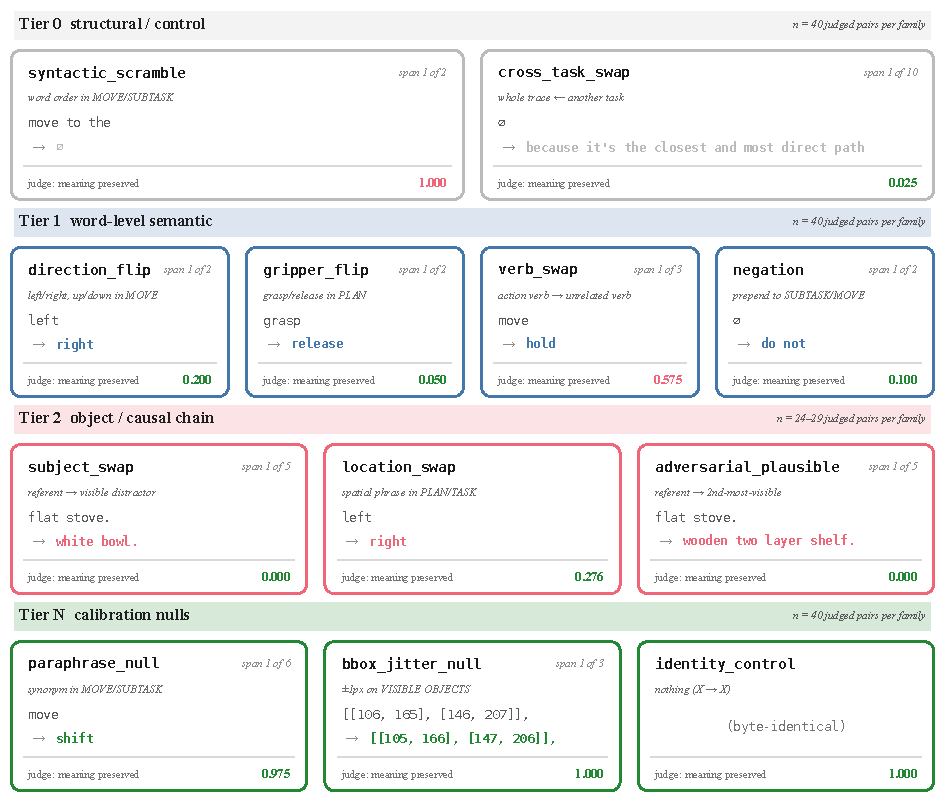
\includegraphics[width=0.996\textwidth]{fig1_task_examples.pdf}
    \caption{\textbf{The edit taxonomy, with the real text each family rewrites.} One panel per family, grouped into the three semantic tiers and the calibration nulls. Every \texttt{monospace} string is generator output from the released edit-pair export; the span shown is recovered by word-level diff of a real (original, edited) pair, not written here; and \emph{span 1 of $k$} says how many spans that trace's edit touched, so a single-span excerpt is not mistaken for the whole edit. The bottom line of each panel is the blind judge's meaning-preserved rate for that family (Section~\ref{sec:judge_edits}). Colour is keyed to intent, not the rate: a high rate is the design for a null and a failure for a semantic family. Two rates are therefore drawn red on purpose: \emph{syntactic\_scramble}, filed in Tier~0 as structural yet judged meaning-preserving at $1.000$, which is what makes it the length-exact floor of Section~\ref{sec:paraphrase_null}, and \emph{verb\_swap} at $0.575$, so four in ten ``verb swaps'' change no meaning. The figure draws $12$ of the $13$ families: \emph{instr\_random\_sub} edits the instruction and leaves the CoT alone, so it has no CoT span to show, and the identity null appears under the judge export's name for it, \emph{identity\_control}.}
    \label{fig:taxonomy}
\end{figure*}


\paragraph{Tier 0 -- surface / control ($\times 3$).} Interventions that should have zero or maximal effect if the metric is well-behaved.
\emph{selfsplice\_control:} identity substitution (X$\to$X). \emph{syntactic\_scramble:} word-order shuffle within \texttt{MOVE} and \texttt{SUBTASK}, preserving content words, and an LLM judge confirms it preserves \emph{meaning} at a rate of $1.000$ (Section~\ref{sec:judge_edits}), so it is best read as a second meaning-preserving family rather than as a structural edit. \emph{cross\_task\_swap:} replace the entire CoT with the reasoning from an unrelated LIBERO sample.

\paragraph{Tier 1 -- word-level semantic ($\times 4$).} Single-token or short-phrase swaps that mutate one semantic axis at a time. \emph{direction\_flip:} left$\leftrightarrow$right, up$\leftrightarrow$down, in$\leftrightarrow$out within \texttt{MOVE}. \emph{gripper\_flip:} grasp$\leftrightarrow$release, open$\leftrightarrow$close within \texttt{PLAN}/\texttt{SUBTASK}. \emph{verb\_swap:} action verbs $\to$ unrelated verbs, though an LLM judge finds the swap actually changes meaning in only $0.575$ of pairs (Section~\ref{sec:judge_edits}), so this family is weaker than its name suggests. \emph{negation:} prepend ``do not'' to \texttt{SUBTASK}/\texttt{MOVE}.

\paragraph{Tier 2 -- object / causal-chain ($\times 3$).} Higher-order edits requiring cross-tag consistency. \emph{subject\_swap:} primary object referent $\to$ visible distractor across all reasoning tags. \emph{location\_swap:} spatial adverbs and 2-word location phrases within \texttt{PLAN}/\texttt{SUBTASK}/\texttt{TASK} (left/right, top/bottom, front/back, near/far, inside/outside, `left compartment' etc.). \emph{adversarial\_plausible:} object $\to$ second-most visible object, \emph{intended} to be visually plausible but wrong. An LLM judge confirms the referent changes ($0.958$) but rejects the plausibility half of that description: only $0.125$ of its edits are judged plausible (Section~\ref{sec:judge_edits}). We keep the family and the name, and readers should treat it as an unconstrained object substitution rather than as an adversarially plausible one.

\paragraph{Tier N -- calibration nulls ($\times 3$).} Meaning-preserving perturbations whose score defines each model's \emph{floor}. Every reported $\mathcal{F}$ must be read against them, and we treat them as first-class families rather than sanity checks. \emph{paraphrase\_null:} synonym substitution within \texttt{MOVE}/\texttt{SUBTASK} that preserves the instruction's meaning (\S~\ref{sec:paraphrase_null}). \emph{bbox\_jitter\_null:} $\pm 1$\,px perturbation of the \texttt{VISIBLE OBJECTS} bounding-box coordinates, below the resolution the reasoning operates at. \emph{instr\_random\_sub:} 5-token random substitution in the \emph{instruction} rather than the CoT, which measures each model's global prompt sensitivity from \emph{outside} the CoT segment and so bounds how much of any CoT-edit score is CoT-specific at all. (\emph{selfsplice\_control} above is the fourth, degenerate null: exact identity, expected and observed $0.00$.)

Total: $\mathbf{10}$ edit families across three semantic tiers (of which \emph{selfsplice\_control} is the degenerate identity null, leaving $9$ non-null), plus $\mathbf{3}$ calibration nulls: $\mathbf{13}$ families in all, matching Table~\ref{tab:compare}. Applied to $N{=}58$--$100$ LIBERO samples per model, with \emph{location\_swap} at $N\!\approx\!58$--$74$ after the annotation fix. \textbf{Coverage:} the calibration nulls have now been run on \textbf{all $\mathbf{11}$ models in the benchmark, in both architecture families} (the seven ``ours'' leaderboard rows at 3 sampling seeds each, ECoT-bridge, an independent retraining of the no-CoT variant, and the three DeepThinkVLA checkpoints), so every $\mathcal{F}$ in Table~\ref{tab:leaderboard} has a measured floor and a measured ceiling from its own run, and the out-of-CoT specificity check is defined on every model (Table~\ref{tab:calibration}). One family is \emph{inapplicable} rather than unmeasured: \emph{bbox\_jitter\_null} perturbs bounding-box coordinates, and DeepThinkVLA's CoT renderer emits no bounding boxes, so the edit yields a byte-identical trace. The harness refuses to score an edit that does not survive rendering and records $n{=}0$ with all $100$ samples skipped, rather than returning the $\mathcal{F}=0.000$ that an unguarded run would report, a number that is indistinguishable from \emph{selfsplice\_control} and would read as robustness where in fact no perturbation reached the model (\S~\ref{sec:f2_calib}).

\subsubsection{Faithfulness Score}

For each sample $s$ and edit family $f$, let $a(s, \text{cot}) \in \mathbb{R}^7$ denote the greedy-decoded action after de-quantising the 7 action tokens. The per-sample per-family faithfulness signal is
\begin{equation}
\Delta_\infty^{s,f} \;=\; \max_{i \in [7]}\bigl|\, a_i(s,\, f(\text{cot}_s)) - a_i(s,\, \text{cot}_s)\,\bigr|,
\label{app:eq:delta}
\end{equation}
where $a_i$ is the $i$-th action dimension normalized to $[-1, 1]$. A sample is \emph{faithful under $f$} iff $\Delta_\infty^{s,f} > \tau$, with $\tau = 0.05$ (5\% of the normalized action range). The \emph{Faithfulness Score} for a model $m$ on family $f$ is
\begin{equation}
\mathcal{F}(m, f) \;=\; \frac{1}{N} \sum_{s=1}^N \mathbf{1}\!\bigl[\Delta_\infty^{s,f}(m) > \tau\bigr].
\label{app:eq:faith}
\end{equation}
The overall Faithfulness Score is $\bar{\mathcal{F}}(m) = \tfrac{1}{|F|}\sum_{f \in F}\mathcal{F}(m, f)$, averaged over the 7 non-control edit families.

\paragraph{Null-control validation (two-fold, \S~\ref{sec:paraphrase_null}).}
\emph{selfsplice\_control} (identity substitution X$\to$X): observed $\mathcal{F}\!=\!0.000$ on 11/11 CoT-VLAs. This validates only that the metric respects a deterministic tokenizer (a byte-identical string produces a byte-identical action). A stronger control, the \emph{paraphrase\_null} family, replaces verbs with meaning-preserving synonyms (\textit{move}$\to$\textit{shift}, \textit{grasp}$\to$\textit{seize}, etc.) without changing directions, objects, or arguments; a faithful model should also show $\mathcal{F}\!\approx\!0$ under this edit, since the semantic content is unchanged. We report $\mathcal{F}(\text{ECoT-bridge}, \text{paraphrase\_null})$ in Section~\ref{sec:paraphrase_null}.

\subsubsection{Attention decomposition}
For an action-token source position $t \in \{T-6, \dots, T\}$, the attention mass on each segment bucket $B \in \{\text{visual}, \text{instruction}, \text{cot}, \text{action-prev}\}$ is
\begin{equation}
\begin{split}
\alpha(m, B) \;=\; \frac{1}{|L|\cdot|H|\cdot 7}
\sum_{\ell \in L}\sum_{h \in H}\\
\sum_{t=T-6}^{T}\sum_{j \in B} A_{\ell,h}^{(t,j)}(m),
\end{split}
\label{eq:attn}
\end{equation}
where $A_{\ell,h}^{(t,j)}$ is the attention weight from action position $t$ to key position $j$, and $L = \{0,1,2,3\}$ (early LLM layers) and $H$ are the 32 attention heads. The choice of $L$ is consequential and not innocent: over all $32$ layers the four buckets reorder (Section~\ref{sec:analysis}), so every $\alpha$ in this paper is an early-layer quantity and we report the full-depth values alongside.

\subsubsection{Evaluation protocol}
\emph{Sample selection.} 100 first-step samples per condition; where compute permits, 3 file-shuffle seeds. \emph{Statistical protocol.} We report mean $\pm$ std across seeds where $\geq 2$ seeds exist, which is now every row of Table~\ref{tab:leaderboard} (all 8 CoT-VLA rows at 3 seeds), and single-run point estimates with Wilson 95\% CIs otherwise (the three DeepThinkVLA runs of Section~\ref{sec:cross_family}); Wilson intervals on the 3-seed rows are computed on counts pooled over seeds. For attention we separate sampling noise ($\sigma \leq 0.094$\,pp over 3 seeds at $N{=}100$) from same-config training-run noise ($0.12$--$1.95$\,pp over seven independent retraining pairs, one for every trained row), and compare model differences against the latter (Section~\ref{sec:analysis}). \emph{Reproducibility.} A single top-level script reproduces every reported cell in $\sim$3h on 8$\times$A100, and \texttt{scripts/\allowbreak{}verify\_\allowbreak{}paper\_\allowbreak{}numbers.py} re-derives each number quoted in this paper from the released JSON and exits non-zero on any mismatch.

% ============================================================
\subsection{Models}
\label{sec:models}
% ============================================================

Table~\ref{tab:models} lists the 15 models across 4 model families, which span 2 base architectures: OpenVLA-7B for A, C and D, PaliGemma for B. Only the \emph{no-CoT} variant differs from our main model in the training \emph{target} (action-only); all other ``ours'' variants share the same nine-tag target. This isolates the effect of reasoning-target training with all other factors held constant.

\begin{table*}[t]
\centering\small
\caption{The 15 models in CoT-Faith across 4 model families. Two base architectures: OpenVLA-7B (A, C, D) and PaliGemma (B), which is what ``both architecture families'' refers to wherever this paper compares across them. ``Ours'' variants LoRA-fine-tuned from \texttt{Embodied-\allowbreak{}CoT/\allowbreak{}ecot-\allowbreak{}openvla-\allowbreak{}7b-\allowbreak{}bridge}.}
\label{tab:models}
\fitwidth{\textwidth}{\begin{tabular}{l l l l l}
\toprule
Model & Base architecture & Training data & LoRA rank & Reasoning target \\
\midrule
\multicolumn{5}{l}{\textit{Family A: OpenVLA non-CoT baselines (4)}} \\
OpenVLA-libero-spatial & OpenVLA-7B     & LIBERO-Spatial & (public FT) & no CoT \\
OpenVLA-libero-object  & OpenVLA-7B     & LIBERO-Object  & (public FT) & no CoT \\
OpenVLA-libero-goal    & OpenVLA-7B     & LIBERO-Goal    & (public FT) & no CoT \\
OpenVLA-libero-10      & OpenVLA-7B     & LIBERO-10      & (public FT) & no CoT \\
\midrule
\multicolumn{5}{l}{\textit{Family B: DeepThinkVLA (3)}} \\
DeepThinkVLA-base      & PaliGemma      & (pretrain only)   & --- & --- \\
DeepThinkVLA-SFT       & PaliGemma      & LIBERO-CoT       & (public) & CoT (SFT) \\
DeepThinkVLA-RL        & PaliGemma      & LIBERO-CoT       & (public) & CoT (RL) \\
\midrule
\multicolumn{5}{l}{\textit{Family C: ECoT (1 public)}} \\
ECoT-bridge            & ECoT-OpenVLA-7B & Bridge-V2       & (public) & full 9-tag CoT \\
\midrule
\multicolumn{5}{l}{\textit{Family D: Ours (7 LoRA variants)}} \\
Ours r=8/16/32/64      & ECoT-bridge & LIBERO-90 & \{8,16,32,64\} & full CoT \\
Ours no-CoT            & ECoT-bridge & LIBERO-90 & 32             & \textbf{action-only} \\
Ours data-50A/B        & ECoT-bridge & LIBERO-90 (50\% split A/B) & 32 & full CoT \\
\bottomrule
\end{tabular}}
\end{table*}

% ============================================================
\subsection{Model scores, and why we do not publish them as a ranking}
\label{sec:results}
% ============================================================

Table~\ref{tab:leaderboard} reports the magnitude score $\mathcal{F}(m, f)$ for every model$\times$family cell we measured: rows are the 8 CoT-VLA models (non-CoT baselines have no CoT to edit and appear only in Fig.~\ref{fig:attention}), columns are the 10 non-null edit families plus one paraphrase-null (\emph{para}, Section~\ref{sec:paraphrase_null}) organized by tier. Fig.~\ref{fig:edit_heatmap} visualizes the same table as a heatmap. \textbf{Every row is a 3-seed mean$\pm$std} of a single 13-family run of that checkpoint, so every cell in the table carries an error bar and the \emph{para} floor is populated on all 8 rows.

\textbf{This table is a diagnostic, not a leaderboard, and the distinction is the paper's main methodological point.} Section~\ref{sec:paraphrase_null} makes a per-model paraphrase floor a \emph{required} field for admission to the public leaderboard. Seven of the eight rows below do not carry one, so \textbf{by our own admission rule seven of our own eight submissions would be rejected}, and the eighth (ECoT-bridge, the only fully calibrated row) has a floor that sits at the same height as its maximum-effect ceiling, which means its cells cannot be read as semantic sensitivity either. There is therefore no subset of this table on which a ranking is licensed, and we publish none: \textbf{no cell is bolded and the row order is the configuration order of Table~\ref{tab:models}, not a score order.} What the table is \emph{for} is the two structural findings it makes visible: that magnitude scores can sit on an unmeasured high floor (F6, Section~\ref{sec:paraphrase_null}) and that they are direction-blind (Section~\ref{sec:directional}, final column). A reader who wants a comparative claim from CoT-Faith should take it from $\mathcal{F}_{\text{dir}}$ or from $\mathcal{F}_{\text{diff}}$, never from the magnitude cells.

\begin{table*}[t]
\centering\scriptsize
\caption{\textbf{Magnitude scores $\mathcal{F}(m, f)$: a diagnostic table, not a ranking.} 8 CoT-VLAs $\times$ 11 edit families (10 non-null + \emph{paraphrase\_null}), with the direction-aware score on \emph{direction\_flip} in the last column. Every row is a \textbf{mean$\pm$std across 3 sampling seeds} of one 13-family run at $N$ as given in the header, so every cell here now carries a floor from its own run; the two out-of-CoT floors are in Table~\ref{tab:calibration} rather than here. \textbf{Nothing is bolded, deliberately}, and the reason is now measured on all 8 rows rather than argued from the 1 we could calibrate: on \emph{every} row the mean over the seven non-control families falls \emph{below} that row's own \emph{para} floor ($\bar{\mathcal{F}}_{\text{diff}}$ from $-0.028$ to $-0.179$; Section~\ref{sec:paraphrase_null}), so a column maximum identifies the model that reacts most to \emph{any} rewording, not the model that is most faithful. Row order is the configuration order of Table~\ref{tab:models}. \emph{ss} $=$ selfsplice\_control (null; observed $0.00$ on 8/8 here, and on 11/11 including the DeepThinkVLA family). This table is the ECoT architecture family only; the second family's full 13-family protocol is Table~\ref{tab:crossfamily} and Table~\ref{tab:calibration}, which is \emph{not} merged in because its floor, ceiling, and decode conventions all differ. \emph{para} $=$ paraphrase\_null, the per-model surface-form floor. $\mathcal{F}_{\text{dir}}$ (Eq.~\ref{eq:fdir}) requires the action to reverse, not merely to move; \textbf{it orders the models oppositely to the magnitude columns} (Section~\ref{sec:directional}). That last column alone is stated on the checkpoint's own de-quantization grid; the magnitude columns are invariant to that choice and the audit proves it (Section~\ref{sec:analysis}). Wilson 95\% CI half-widths on the pooled 3-seed counts are $\leq 0.067$ (widest: \emph{subject\_swap} on $r{=}64$), but they bound the \emph{sample} draw only, and they are the \emph{smaller} term: retraining $r{=}32$ at the same configuration moves a single family by up to $0.180$, ${\sim}2.7\times$ the widest interval here (Section~\ref{sec:limitations}\,(viii)).}
\label{tab:leaderboard}
\fitwidth{\textwidth}{\begin{tabular}{l r r r r r r r r r r r | r}
\toprule
& \multicolumn{3}{c}{Tier 0 (control)} & \multicolumn{4}{c}{Tier 1 (word-level)} & \multicolumn{3}{c}{Tier 2 (object/causal)} & & \\
\cmidrule(lr){2-4}\cmidrule(lr){5-8}\cmidrule(lr){9-11}
Model & ss & scram. & cross & dir. & grip. & verb & neg. & subj. & loc. & adv. & para. & $\mathcal{F}_{\text{dir}}$ \\
$N=$ & 69 & 100 & 100 & 100 & 100 & 100 & 100 & 69 & 74 & 69 & 100 & 100 \\
\midrule
Ours r=8       & 0.00 & .41\tiny{$\pm .03$} & .86\tiny{$\pm .01$} & .70\tiny{$\pm .04$} & .11\tiny{$\pm .01$} & .64\tiny{$\pm .05$} & .67\tiny{$\pm .04$} & .32\tiny{$\pm .09$} & .10\tiny{$\pm .06$} & .31\tiny{$\pm .07$} & .59\tiny{$\pm .03$} & 0.65\tiny{$\pm .02$} \\
Ours r=16      & 0.00 & .44\tiny{$\pm .01$} & .88\tiny{$\pm .03$} & .75\tiny{$\pm .03$} & .17\tiny{$\pm .03$} & .68\tiny{$\pm .03$} & .66\tiny{$\pm .04$} & .37\tiny{$\pm .06$} & .14\tiny{$\pm .02$} & .36\tiny{$\pm .06$} & .55\tiny{$\pm .04$} & 0.67\tiny{$\pm .05$} \\
Ours r=32      & 0.00 & .35\tiny{$\pm .04$} & .81\tiny{$\pm .02$} & .65\tiny{$\pm .02$} & .13\tiny{$\pm .01$} & .59\tiny{$\pm .01$} & .59\tiny{$\pm .02$} & .33\tiny{$\pm .03$} & .13\tiny{$\pm .04$} & .33\tiny{$\pm .01$} & .57\tiny{$\pm .02$} & 0.58\tiny{$\pm .03$} \\
Ours r=64      & 0.00 & .47\tiny{$\pm .05$} & .89\tiny{$\pm .05$} & .82\tiny{$\pm .02$} & .17\tiny{$\pm .06$} & .84\tiny{$\pm .04$} & .78\tiny{$\pm .03$} & .40\tiny{$\pm .05$} & .22\tiny{$\pm .02$} & .37\tiny{$\pm .02$} & .66\tiny{$\pm .02$} & 0.78\tiny{$\pm .02$} \\
Ours no-CoT    & 0.00 & .15\tiny{$\pm .05$} & .26\tiny{$\pm .03$} & .27\tiny{$\pm .04$} & .07\tiny{$\pm .01$} & .16\tiny{$\pm .04$} & .20\tiny{$\pm .07$} & .16\tiny{$\pm .03$} & .12\tiny{$\pm .05$} & .18\tiny{$\pm .06$} & .19\tiny{$\pm .05$} & 0.09\tiny{$\pm .02$} \\
Ours data-50A  & 0.00 & .39\tiny{$\pm .04$} & .73\tiny{$\pm .03$} & .70\tiny{$\pm .02$} & .12\tiny{$\pm .03$} & .65\tiny{$\pm .04$} & .57\tiny{$\pm .03$} & .30\tiny{$\pm .04$} & .10\tiny{$\pm .02$} & .32\tiny{$\pm .03$} & .54\tiny{$\pm .06$} & 0.64\tiny{$\pm .01$} \\
Ours data-50B  & 0.00 & .35\tiny{$\pm .03$} & .73\tiny{$\pm .07$} & .64\tiny{$\pm .02$} & .15\tiny{$\pm .01$} & .54\tiny{$\pm .02$} & .51\tiny{$\pm .02$} & .28\tiny{$\pm .05$} & .10\tiny{$\pm .03$} & .26\tiny{$\pm .04$} & .45\tiny{$\pm .03$} & 0.54\tiny{$\pm .01$} \\
ECoT-bridge & 0.00 & .86\tiny{$\pm .04$} & .96\tiny{$\pm .01$} & .96\tiny{$\pm .01$} & .70\tiny{$\pm .02$} & .95\tiny{$\pm .04$} & .95\tiny{$\pm .01$} & .93\tiny{$\pm .03$} & .59\tiny{$\pm .05$} & .93\tiny{$\pm .03$} & .95\tiny{$\pm .02$} & 0.12\tiny{$\pm .04$} \\
\bottomrule
\end{tabular}}
\end{table*}

\begin{figure*}[t]
    \centering
    
\includegraphics[width=0.97\textwidth]{fig3_edit_heatmap.pdf}
    \caption{\textbf{The same magnitude scores as a heatmap, all 13 families.} This is Table~\ref{tab:leaderboard}, not a ranking; colour encodes magnitude sensitivity only. Columns are grouped as the axis says: the $7$ \emph{semantic} families (the \texttt{NON\_CONTROL} set \texttt{derive\_metrics.py} averages $\bar{\mathcal{F}}$ over, imported by the generator rather than retyped), the $3$ Tier-0 controls, and the $3$ calibration columns: two floors and the out-of-CoT ceiling. \emph{An earlier version of this figure drew $11$ of the $13$ and did not say so.} The two it omitted are \emph{bbox\_jitter\_null} and \emph{instr\_random\_sub}, both measured on all seven ``ours'' rows; they are also the tightest floor in the paper ($0.05$--$0.09$) and the ceiling every CoT family is compared against, so their absence left a grid with no low column except the identity null and removed the figure's own evidence that the score is not simply always-high. Its axis label promised ``semantic $\to$ controls'' over an order that put the identity null in column $8$. Both are fixed here. The two ECoT-bridge cells with no run print as ``---'' rather than as a colour. \textcolor[HTML]{EE6677}{no-CoT} row collapses across every semantic edit despite identical base and data; \textcolor[HTML]{228833}{ECoT-bridge} row is near-uniformly high. Selfsplice column is $0.00$ across all models (identity-null validation). Note that the ECoT-bridge row's uniformity is precisely the problem F6 and Section~\ref{sec:paraphrase_null} identify: it is also near-uniformly high on the \emph{paraphrase} null, and it drops to $0.12$ under direction-aware scoring. Colour here encodes magnitude sensitivity, not semantic faithfulness.}
    \label{fig:edit_heatmap}
\end{figure*}

\begin{figure*}[t]
    \centering
    
\includegraphics[width=0.98\textwidth]{fig2_attention_distribution.pdf}
    \caption{\textbf{Attention distribution across 15 models spanning 4 model families (P1).} Panel (a): 12 models in the OpenVLA/ECoT families, where the four buckets are directly comparable. All 8 ECoT-family CoT-VLAs (including the reasoning-target-stripped no-CoT variant) cluster tightly at $(\text{visual}, \text{instr}, \text{CoT}, \text{prev}) \approx (0.29, 0.30, 0.34, 0.07)$; OpenVLA non-CoT baselines cluster at $(0.52, 0.42, 0.00, 0.05)$. Panel (b): DeepThinkVLA family (PaliGemma), all four buckets. An earlier version of this panel omitted the visual bar because our harness reported visual~$\equiv 0$; that was a prompt-format bug on our side, not a property of these checkpoints. We had located segment boundaries by searching the decoded prompt for \texttt{"Instruction:"} and \texttt{"Action:"}, neither of which occurs in this model's actual prompt (\texttt{"<image>"}$\times n$ + think-prefix + \texttt{"Task: <instr>;"}), and the not-found fallback collapsed the instruction span. The corrected harness segments on token ids and raises if any boundary is absent; it measures visual at $0.176$ (base) and $0.186$ (SFT/RL). Within DT the CoT bucket rises from $0.119$ (base) to $0.197$ (SFT) and $0.196$ (RL), a training-induced $+7.9$\,pp shift, but $\alpha(\text{cot})$ is \emph{never} the largest bucket on any DeepThinkVLA checkpoint (\texttt{action\_prev} leads on base at $0.384$; \texttt{instr} leads on SFT and RL at $0.310$). Read with the layer-depth sweep below, the ``CoT bucket is largest'' observation is specific to both the layer set \emph{and} the architecture family, and is not a general property of CoT-VLAs. Panel (c): the same records with every bucket divided by its own token count, on the 8 checkpoints where a CoT segment exists. \emph{An earlier version of this caption described panels (a) and (b) and stopped}, leaving the figure's third panel, the one that undoes panel (a)'s headline, unexplained; and its title printed the 8-model \emph{mean} ratio as $4.0\times$ next to a paragraph quoting $3.9\times$ for \emph{r=32}, two correct numbers for two different quantities rounded apart. The panel now prints the range: instruction tokens draw $3.7$--$4.2\times$ more attention each than CoT tokens on \emph{every one} of the 8, which contains the $3.9\times$ Section~\ref{sec:analysis} quotes for \emph{r=32}. The tallest bars are \texttt{action\_prev}, at $8.1\times$ the per-token CoT rate on \emph{r=32}: on a per-token basis this architecture concentrates on the $7$ previous-action tokens, not on its reasoning. The axis is logarithmic because the four buckets span an order of magnitude.}
    \label{fig:attention}
\end{figure*}

% ============================================================
\subsection{Analysis}
\label{sec:analysis}
% ============================================================

We now use CoT-Faith to answer five questions about manipulation CoT-VLAs: three (F1--F3) that admit controlled comparisons under our benchmark, one (O4) that we treat as an uncontrolled observation because two axes are confounded, and one (F5) on cross-corpus transfer at $N{=}100$. Section~\ref{sec:directional} then re-examines all of them under a direction-aware scoring rule, which reverses the leaderboard ordering.

\begin{table*}[t]
\centering\small
\caption{\textbf{P3 re-run in-domain} (\texttt{ecot-openvla-7b-bridge} on Bridge~V2, its training corpus; $N{=}153$, CoT self-generated, prediction un-normalized with the checkpoint's own \texttt{bridge\_orig} statistics). Raw Mann--Whitney AUROC of each attention channel as a predictor of above-median action L$_1$, with a $10{,}000$-draw bootstrap CI over samples. The last column is the same quantity recomputed on the \emph{same forward passes} under the withdrawn mixed-space protocol. Only $\alpha(m,\text{instruction})$ excludes chance, and the withdrawn protocol is what hid it. Artifact: \texttt{results\_\allowbreak{}v2/\allowbreak{}canonical\_\allowbreak{}runs/\allowbreak{}auroc\_\allowbreak{}ecot\_\allowbreak{}bridge\_\allowbreak{}indomain\_\allowbreak{}n153.json}.}
\label{tab:p3}
\fitwidth{\textwidth}{\begin{tabular}{l r l l r}
\toprule
Attention channel & AUROC & 95\% CI & vs.\ chance & withdrawn \\
\midrule
$\alpha(m, \text{cot})$        & $0.596$ & $[0.491, 0.679]$ & includes $0.5$ & $0.531$ \\
$\alpha(m, \text{visual})$     & $0.454$ & $[0.357, 0.564]$ & includes $0.5$ & $0.427$ \\
$\alpha(m, \text{instruction})$& $\mathbf{0.362}$ & $\mathbf{[0.284, 0.469]}$ & \textbf{excludes} $\mathbf{0.5}$ & $0.492$ \\
$\alpha(m, \text{action-prev})$& $0.541$ & $[0.446, 0.633]$ & includes $0.5$ & $0.550$ \\
\midrule
\multicolumn{2}{l}{Median action L$_1$ (robot units)} & $0.0199$ & \multicolumn{2}{l}{withdrawn: $0.2550$ ($12.8\times$)} \\
\multicolumn{2}{l}{Labels differing between protocols} & $40/153$ & \multicolumn{2}{l}{} \\
\bottomrule
\end{tabular}}
\end{table*}


\subsubsection{F5: attention profile and causal-edit response are cross-corpus consistent (N=100 per non-LIBERO corpus)}
\label{sec:cross_corpus}

We ran the ECoT-bridge model on 3 additional manipulation corpora spanning distinct embodiments: Bridge~V2 (WidowX bimanual home, $N{=}100$), RT-1/Fractal (Google office robot, $N{=}100$), BC-Z (everyday manipulation, $N{=}100$). Because these corpora do not carry ground-truth CoT annotations, we let the model self-generate its 9-tag CoT via greedy decode, then apply the same edit protocol. These runs replace an $N{=}30$ pilot, and the replacement is the reason the transfer claim is now worth making: \textbf{every attention bucket mean moves by at most $0.3$\,pp between the two $N$}, so the stability was not a small-sample artifact. The pilot is retained under \texttt{results\_v2/superseded/}.

\textbf{Attention profile is remarkably stable across corpora.} Per-corpus $(\text{visual}, \text{instr}, \text{cot}, \text{prev})$ mean$\pm$std, $N{=}100$ everywhere (BC-Z contributes $99$ usable attention records of its $100$ samples): LIBERO $(.290, .301, .343, .065)$ $\pm(.006, .009, .009, .002)$; Bridge~V2 $(.296, .299, .338, .067)$ $\pm(.010, .012, .017, .004)$; Fractal $(.291, .302, .335, .073)$ $\pm(.008, .010, .014, .004)$; BC-Z $(.297, .310, .323, .070)$ $\pm(.010, .014, .022, .004)$. \textbf{Max deviation across corpora is $\leq 2.1$\,pp on any bucket}: BC-Z's CoT bucket, $2.07$\,pp below LIBERO's, is the largest, \textbf{and every other bucket on every corpus is within $0.9$\,pp.} The LIBERO reference row is the 3-seed \emph{ecot-bridge} profile the rest of the paper uses, so this table and Section~\ref{sec:results} cannot disagree.

\textbf{Causal-edit response also transfers, and at this $N$ the spread narrows.} On direction\_flip: LIBERO $\mathcal{F}\!=\!0.963$ ($N{=}100$), Bridge~V2 $0.913$ ($N{=}92$), Fractal $0.974$ ($N{=}77$), BC-Z $0.951$ ($N{=}81$), a range of $0.06$ across four corpora, where the $N{=}30$ pilot's $1.00$/$0.92$/$0.92$ spanned $0.08$ on $N{=}25$--$26$ apiece. On gripper\_flip: LIBERO $0.697$, Bridge~V2 $0.804$ ($N{=}51$), Fractal $0.770$ ($N{=}74$), BC-Z $0.746$ ($N{=}63$). The per-family $N$ is what the visibility gate admits, and it is $2$--$4\times$ the pilot's on every cell. \textbf{F5: Both the attention profile and the primary causal-edit responses of a CoT-VLA transfer cross-corpus at $N{=}100$; CoT-Faith metrics can serve as portable diagnostics across embodiments.} What F5 does \emph{not} say, and Section~\ref{sec:directional} makes explicit: these are \emph{magnitude} responses, and it is exactly the magnitude score that Section~\ref{sec:f2_calib} shows is uninterpretable without its floor. The nulls were not run on these corpora, so F5 is a portability result for the \emph{pipeline}, not evidence that the CoT drives the action on any of them.

\begin{figure*}[t]
    \centering
    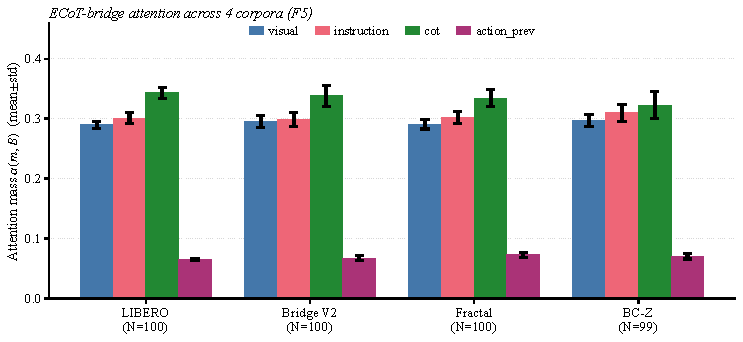
\includegraphics[width=0.783\textwidth]{fig7_cross_corpus.pdf}
    \caption{\textbf{Cross-corpus attention profile (F5, $N{=}100$ per non-LIBERO corpus).} ECoT-bridge evaluated on LIBERO (LIBERO-90, $N{=}100$) and on Bridge~V2, RT-1/Fractal, and BC-Z at $N{=}100$ each (self-decoded CoT; BC-Z yields $99$ usable attention records). Error bars are $\pm 1$ std across samples. Max deviation on any bucket is $\leq 2.1$\,pp. \emph{Both the bars and the error bars are each run's own aggregate over all of its attention records, and the release ships the first $20$ of those records per run rather than all $100$}: recomputing this figure from the released per-sample records reproduces every bucket to within $0.37$\,pp and the bucket ordering exactly, but not the printed digits. The truncation and what it costs a re-deriver are stated in full in the release paragraph of Section~\ref{sec:limitations}. Replaces an $N{=}30$ pilot whose every bucket mean this run reproduces to within $0.3$\,pp; the pilot is retained under \texttt{results\_v2/superseded/}.}
    \label{fig:cross_corpus}
\end{figure*}

\begin{figure*}[t]
    \centering
    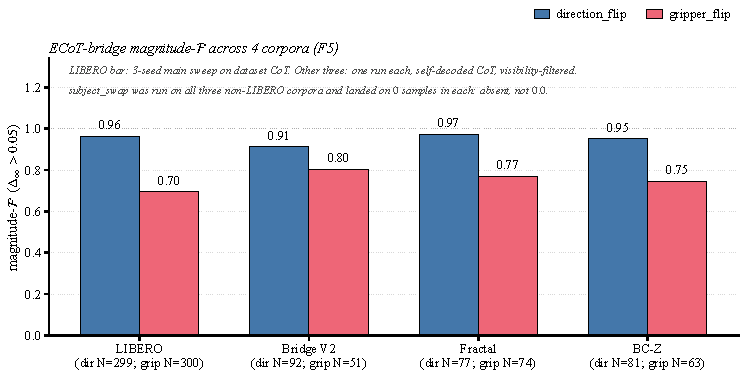
\includegraphics[width=0.786\textwidth]{fig10_cross_corpus_edit.pdf}
    \caption{\textbf{Cross-corpus causal-edit response (F5, $100$ samples requested per non-LIBERO corpus).} ECoT-bridge direction\_flip / gripper\_flip magnitude response on LIBERO and on Bridge~V2, Fractal, BC-Z (self-decoded CoT, $N{=}51$--$92$ after visibility filtering, against $N{=}15$--$26$ in the superseded $N{=}30$ pilot). \emph{Two disclosures the earlier caption did not carry.} (i) The LIBERO bar is not the same kind of measurement as the other three: it is the $3$-seed main sweep on the corpus's own CoT annotations, over $N{=}299$ and $N{=}300$ records; the earlier caption's ``LIBERO ($N{=}100$)'' was the per-seed sample count, not what the bar averages. The other three are one run each of self-decoded CoT. The protocol split is printed on the figure. (ii) A third family, subject\_swap, was run on all three non-LIBERO corpora and landed on $0$ samples in every one; the figure says so rather than dropping it, because ``ran and never applied'' is not the same claim as ``not run'', and neither is $\mathcal{F}{=}0$. Note also that these are \emph{magnitude} scores; the direction-aware scores of Section~\ref{sec:directional} do not transfer in the same way, and the calibration nulls were not run on these corpora, so no floor-corrected statement is available for them. Reports: \texttt{results\_\allowbreak{}v2/\allowbreak{}canonical\_\allowbreak{}runs/\allowbreak{}cross\_\allowbreak{}corpus\_\allowbreak{}\{\allowbreak{}bridge\_\allowbreak{}v2,\allowbreak{}fractal,\allowbreak{}bcz\}\_\allowbreak{}n100.json}.}
    \label{fig:cross_corpus_edit}
\end{figure*}

\begin{figure*}[t]
    \centering
    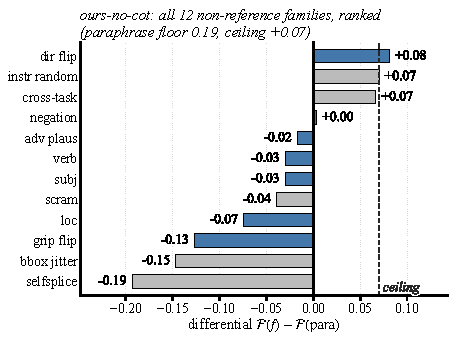
\includegraphics[width=0.98\textwidth]{fig12_directional_inversion.pdf}
    \caption{\textbf{F6: the leaderboard inverts under direction-aware scoring.} \emph{(a)} $\mathcal{F}_{\text{mag}}$ (solid) against $\mathcal{F}_{\text{dir}}$ (hatched) on \emph{direction\_flip}, 3-seed means: the two scores track each other on the six LoRA/data variants and come apart completely on the two ends: ECoT-bridge $0.96 \to 0.12$ and no-CoT $0.27 \to 0.09$. \emph{(b)} The signed translation cosine that produces the gap, over all samples and over the subset Eq.~\ref{app:eq:faith} counts as faithful; the faithful target is $-1$. Only the six full-CoT variants are on the correct side of zero, and they move further toward the target on exactly the samples magnitude-scoring credits. \emph{(c)} $\mathcal{F}_{\text{diff}} = \mathcal{F}(f) - \mathcal{F}(\text{paraphrase\_null})$ for \emph{ours-no-CoT}, the model whose floor ($0.19$) is low enough for the differential to be readable; now all $12$ non-reference families, ranked. \emph{An earlier version of this panel drew $9$ of them}, and the three it omitted are the three that set the scale: \emph{selfsplice\_control} at $-0.193$ (the identity null, which is minus the floor by construction), \emph{bbox\_jitter\_null} at $-0.147$, and \emph{instr\_random\_sub} at $+0.070$, the deliberately random instruction substitution, i.e.\ the \emph{ceiling}. With the ceiling drawn, the panel's content is that the entire floor-to-ceiling band is $0.07$ wide: $8$ of the $12$ families sit below their own floor, the four that clear it do so by $\leq 0.081$, and \emph{direction\_flip}'s $+0.081$ is \emph{above the ceiling}: a meaning-changing edit moves this model no further than substituting a random instruction does. Semantic families are drawn in colour and controls/calibrators in grey; they interleave. Generated by \texttt{figures/\allowbreak{}gen\_\allowbreak{}fig12\_\allowbreak{}directional\_\allowbreak{}inversion.py} from \texttt{derived\_metrics.json}.}
    \label{fig:directional}
\end{figure*}

\begin{table*}[t]
\centering\small
\caption{\textbf{Two-sided calibration on all eleven models we can calibrate, spanning both architecture families.} Every quantity in a row is computed only against families from that same run, so no cross-run offset enters. The seven \emph{Ours} leaderboard rows are 3-sampling-seed means (per-family $F$ averaged over seeds, Wilson intervals on pooled counts); the remaining rows (ECoT-bridge, the no-CoT replicate, and the three DeepThinkVLA checkpoints) are single-seed calibration runs and are marked $^\dagger$. \emph{Ours no-CoT} appears twice and the two rows are not interchangeable: \emph{(leaderboard)} is the checkpoint every other table uses, \emph{(replicate)} is an independent training of the same configuration, and the gap between their two-sided scores ($-0.416$ vs.\ $+0.127$) is itself the training-run variance of item~(viii). \textbf{The \emph{bbox} cell is empty on the DeepThinkVLA rows because that family is inapplicable to them, not unmeasured}: their CoT renderer emits no bounding boxes, so the edit produces a byte-identical trace and the harness records $n{=}0$ with all $100$ samples skipped rather than scoring an identity edit as $\mathcal{F}=0.000$. Dynamic range $=$ ceiling $-$ floor; a range below $0.05$ makes the two-sided statistic undefined and is marked \emph{degen.} Specificity ratio $= \bar{\mathcal{F}} / \mathcal{F}(\text{instr\_rand})$, where $\bar{\mathcal{F}}$ is the mean over the seven non-control families; $>\!1$ means the CoT families move the action more reliably than corrupting five \emph{instruction} tokens does.}
\label{tab:calibration}
\fitwidth{\textwidth}{\begin{tabular}{lcccccrrr}
\toprule
model & $\bar{\mathcal{F}}$ & $\mathcal{F}(\text{para})$ & $\mathcal{F}(\text{bbox})$ & $\mathcal{F}(\text{instr\_rand})$ & ceiling & range & two-sided & ratio \\
\midrule
Ours r=8              & $0.407$ & $0.587$ & $0.077$ & $0.333$ & $0.857$ & $0.270$ & $-0.665$ & $1.222$ \\
Ours r=16             & $0.446$ & $0.547$ & $0.083$ & $0.437$ & $0.883$ & $0.337$ & $-0.299$ & $1.022$ \\
Ours r=32             & $0.395$ & $0.567$ & $0.073$ & $0.370$ & $0.810$ & $0.243$ & $-0.706$ & $1.067$ \\
Ours r=64             & $0.514$ & $0.657$ & $0.087$ & $0.500$ & $0.887$ & $0.230$ & $-0.621$ & $1.028$ \\
Ours no-CoT (leaderboard)          & $0.166$ & $0.193$ & $0.047$ & $0.263$ & $0.260$ & $0.067$ & $-0.416$ & $0.629$ \\
Ours no-CoT (replicate)$^\dagger$  & $0.124$ & $0.110$ & $0.050$ & $0.190$ & $0.220$ & $0.110$ & $\mathbf{+0.127}$ & $0.653$ \\
Ours data-50A         & $0.393$ & $0.537$ & $0.067$ & $0.433$ & $0.730$ & $0.193$ & $-0.743$ & $0.907$ \\
Ours data-50B         & $0.353$ & $0.447$ & $0.053$ & $0.270$ & $0.733$ & $0.287$ & $-0.327$ & $1.307$ \\
ECoT-bridge$^\dagger$ & $0.869$ & $0.960$ & $0.460$ & $0.990$ & $0.970$ & $\mathbf{0.010}$ & \emph{degen.} & $0.878$ \\
\midrule
\multicolumn{9}{l}{\emph{Second architecture family (PaliGemma / \texttt{pi0fast\_base}, single \texttt{<think>} block, $(10,7)$ chunk decode)}} \\
DeepThinkVLA-base$^\dagger$ & $0.947$ & $0.960$ & --- & $0.950$ & $0.980$ & $\mathbf{0.020}$ & \emph{degen.} & $0.996$ \\
DeepThinkVLA-SFT$^\dagger$  & $0.701$ & $0.810$ & --- & $0.870$ & $0.960$ & $0.150$ & $-0.728$ & $0.806$ \\
DeepThinkVLA-RL$^\dagger$   & $0.724$ & $0.820$ & --- & $0.890$ & $0.940$ & $0.120$ & $-0.796$ & $0.814$ \\
\bottomrule
\end{tabular}}
\end{table*}

\begin{table*}[t]
\centering
\small
\caption{\textbf{P2 on the DeepThinkVLA family (F7).} $\bar{\mathcal{F}}$ is the mean over the 7 non-control families. The floor is \emph{paraphrase\_null} (meaning-preserving), the ceiling \emph{cross\_task\_swap} (CoT replaced by an unrelated task's). ECoT-bridge is repeated from Section~\ref{sec:f2_calib} for comparison. $\mathcal{F}_{\text{diff}} < 0$ on \emph{every} model with a measured floor: a paraphrase that changes no meaning moves the action \emph{more} than the mean semantic edit does.}
\label{tab:crossfamily}
\fitwidth{\textwidth}{\begin{tabular}{lccccc}
\toprule
model & $\bar{\mathcal{F}}$ & floor & ceiling & range & $\bar{\mathcal{F}}_{\text{diff}}$ \\
\midrule
DeepThinkVLA-base & $0.947$ & $0.960$ & $0.980$ & $0.020$ & $-0.013$ \\
DeepThinkVLA-SFT  & $0.701$ & $0.810$ & $0.960$ & $0.150$ & $-0.109$ \\
DeepThinkVLA-RL   & $0.724$ & $0.820$ & $0.940$ & $0.120$ & $-0.095$ \\
\midrule
ECoT-bridge (\S\ref{sec:f2_calib}) & $0.869$ & $0.960$ & $0.970$ & $0.010$ & $-0.091$ \\
\bottomrule
\end{tabular}}
\end{table*}

\subsection{Discussion and limitations}
\label{sec:limitations}
% ============================================================

\begin{figure*}[t]
    \centering
    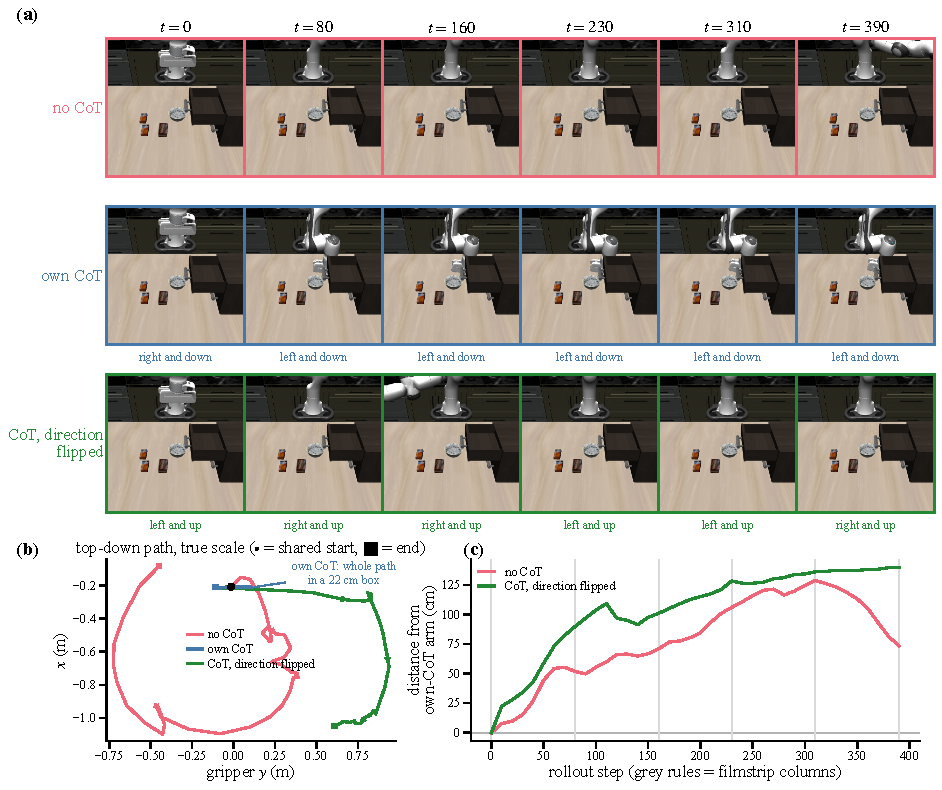
\includegraphics[width=\textwidth]{fig15_rollout_filmstrip.pdf}
    \caption{\textbf{The first run of this harness whose arms are paired at the pixel level, and the only picture in this paper of what a CoT edit does to a trajectory rather than to one decode.} One episode (\emph{libero\_90} task ``close the top drawer of the cabinet'', task~$0$/episode~$0$) with three arms replayed from one init state for $400$ steps, the CoT regenerated \emph{every} step. \textbf{(a)} the frame as the policy saw it, at $t = 0, 80, 160, 230, 310, 390$: the capture stores one frame every $10$ steps, so the columns are the stored frames nearest to even spacing over the $400$ and not exactly even ones; beneath each CoT row is the MOVE phrase that step's reasoning actually carried, so the instruction the policy read is printed next to the motion it produced (the flipped row reads ``left and up'' at $t{=}0$ where the clean row reads ``right and down''). All three rows are the same pixels at $t{=}0$ (max mean $|\Delta\text{pixel}| = 0.0$), which is what the four pairing fixes above bought, and which the generator verifies before it draws rather than after. \textbf{(b)} the top-down gripper path, \emph{at true scale}: one metre scale on both axes, so the box the own-CoT arm never leaves can be read directly against the loops the other two make, and laid on its side ($y$ across, $x$ up) because on an equal aspect these three tracks are a portrait shape. Arrowheads give the direction of travel, the filled square each arm's last recorded pose, and the black dot the start all three share. The arm reading its \emph{own} reasoning is the one that barely travels: its whole path fits in a $21.8$\,cm box, while both other arms cross the workspace. \textbf{(c)} per-step distance from the clean-CoT arm, which peaks at $139.7$\,cm for the flipped arm and $128.8$\,cm for the no-CoT arm, and the peak is not the end, since the no-CoT arm loops back to $73.5$\,cm by $t{=}390$ while the flipped arm finishes at its furthest ($139.6$\,cm). \textbf{None of this is a faithfulness measurement.} All three arms score $0$, so no $\Delta$SR is defined (item~(v)), and one episode of one task supports no ranking of anything. What it does establish is that a CoT edit reaches the actuator and keeps moving the arm for hundreds of steps, a claim every $\Delta_\infty$ in this paper makes at step $0$ and none of them could show over a trajectory. Between-column change \emph{within} an arm runs $0.04$--$7.7$ absolute pixel levels (means $2.4$--$3.8$), so two near-identical adjacent cells are a policy that has stalled and not a repeated frame. Drawn by \texttt{figures/\allowbreak{}gen\_\allowbreak{}fig15\_\allowbreak{}rollout\_\allowbreak{}filmstrip.py} from \texttt{results\_\allowbreak{}v2/\allowbreak{}canonical\_\allowbreak{}runs/\allowbreak{}rollout\_\allowbreak{}filmstrip/\allowbreak{}} (compute-platform \texttt{9r2mm3n3na}); every number in this caption is read back out of that directory's \texttt{fig15\_facts.json} by the audit.}
    \label{fig:filmstrip}
\end{figure*}

\subsection{Sections deferred to the full-length manuscript}
\label{sec:deferred}
The submitted PDF is capped at $20$ pages. These sections of the full-length
manuscript are therefore not reproduced above; they are in the released source
(\texttt{cot\_faith\_iclr.tex}), which is the document the audit script checks
claim by claim and the document every line above was copied from. They are
named here so that a reader can tell what exists from what was cut, and no
claim in the body rests on one of them:
Per-task decomposition: the below-floor result is not an artefact of averaging\label{sec:per_task}; Introduction; Related work; Per-token normalization: the CoT bucket is the largest only because it is the longest; Attention noise, decomposed; The bucket ordering is an artifact of the layer choice; The gate also fails on our own checkpoint, and that constrains how Table~\ref{tab:leaderboard} may be read; The rollout gate: four failures, three causes, and a pass; The gate passes, and both corrections are necessary for it to; The decode defect is on the rollout path, so we measured whether it reaches the published numbers, rather than asserting that it does not; Norm-stats provenance, and why the rollout-level CoT edit cannot use the public CoT checkpoint; The blocker on that ablation is not compute, and we measured what it is; Is the floor itself confounded with sequence length? Yes, and swapping it does not rescue the metric, it inverts the sign; All eleven calibrated models, in both architecture families: the degeneracy tracks saturation, and the specificity check splits; Ancillary: prompt-format ablation; Threshold and metric sensitivity; What is missing; $\mathcal{F}_{\text{dir}}$, unlike $\mathcal{F}_{\text{mag}}$, has a null it clears, and it correctly fails the no-CoT control; O4 (observation, not a controlled finding): a Bridge-corpus CoT-VLA is $\sim 2\times$ more faithful, but the comparison confounds two axes\label{sec:o4}; F1: Attention on CoT is a floor set by architecture; training induces only a small shift; F2: Causal effect requires reasoning-target training; F2 calibrated: the no-CoT collapse is a uniform gain reduction, not selective CoT-insensitivity\label{sec:f2_calib}; F3: Attention distribution does not predict causal effect; F6: magnitude-based edit scoring inverts the model ordering; Attention-as-failure AUROC (P3): specified, withdrawn, and re-run in-domain; Paraphrase-null: models are sensitive to surface tokens, not just meaning\label{sec:paraphrase_null}; Do the edit families do what their names say? An LLM-judge validation of the generators\label{sec:judge_edits}; F7: P2 on a second architecture family; the construct-validity failure replicates, and worsens\label{sec:cross_family}; P3, re-run in-domain: correcting the protocol does not recover a predictor\label{sec:p3_indomain}; Limitation (v), measured: does the token-level score predict what the arm does?\label{sec:deltapath}.


\end{document}
